\documentclass[11pt]{article}

% ==========================================
% PACKAGES
% ==========================================
\usepackage[margin=1in]{geometry}
\usepackage{cite}
\usepackage{amsmath,amssymb,amsfonts}
\usepackage{algorithmic}
\usepackage{algorithm}
\usepackage{graphicx}
\usepackage{textcomp}
\usepackage{xcolor}
\usepackage{array}
\usepackage{booktabs}
\usepackage{multirow}
\usepackage{tikz}
\usetikzlibrary{automata,positioning,arrows.meta}
\usepackage{placeins}
\usepackage{forest}
\usepackage{microtype}
\usepackage[hidelinks]{hyperref}
\usepackage{titlesec}
\usepackage{parskip}

% Build switches and shared macros.
% Build switches. \drafttrue renders \pending{...} in red; with \draftfalse an
% unresolved \pending stops the build, so none can reach a submission PDF.
% \testbedBtrue adds the Testbed B text (the prover-scaling runs exist; the composite and load runs are still \pending).
\newif\ifdraft \drafttrue
\newif\iftestbedB \testbedBtrue
\newcommand{\pending}[1]{\ifdraft\textcolor{red}{[PENDING: #1]}\else
  \PackageError{engram}{Unresolved pending: #1}{Resolve it before a final build.}\fi}

% Numbered results: \refstepcounter{...}\label{...} before the bold heading makes
% every \ref clickable and keeps the numbers in step with the text.
\newcounter{lemma}
\newcounter{corollary}
\newcounter{theorem}
\newcounter{definition}

% Numbers quoted in more than one place. Each value is the one reported in the
% table or section named beside it; change it here and every quotation follows.
\newcommand{\resFSMStatesM}{2.13 million}      % Table~\ref{tab:formal-verification}, FSM (safety)
\newcommand{\resFSMStatesExact}{2{,}126{,}591} % same row, exact count
\newcommand{\resAblationCount}{five}           % rows of Table~\ref{tab:ablation}
\newcommand{\resProposalBytes}{894}            % Txs[0] certificate bytes at 7 validators, live mean in ANCHORED (certificate_size_scan.py); size = 70 + 118 n
\newcommand{\resValidationUs}{301}             % ProcessProposal on an accepted proposal, 7 validators, microseconds (10 runs, sd 13; tests/benchmark)
\newcommand{\resExtendVoteMs}{16.6}            % mean ExtendVote time, milliseconds
\newcommand{\resBlockEngram}{1.262}            % Table~\ref{tab:overhead}, Engram block interval, s
\newcommand{\resBlockVanilla}{1.233}           % Table~\ref{tab:overhead}, 7 validators without extensions, s
\newcommand{\resOverheadPct}{1.8\%}              % paired estimate of Engram's addition over the seven-validator arm (20 pairs)
\newcommand{\resOverheadCI}{0.4 to 3.1\%}   % 95\% interval (Student t) of the paired estimate, 20 pairs (scripts/e7_consensus_overhead/paired_overhead.py)
\newcommand{\resRQTwoEngram}{96--100\%}         % Table~\ref{tab:rq2}: Engram's block count against its healthy rate, across faults (cell means)
\newcommand{\resRQTwoOob}{20--61\%}           % same table: the receipt-gated baseline that reads the layers at each validator (cell means)
\newcommand{\resInBandHalt}{44--121}          % seconds after the fault began at which the vote-extension baseline stopped committing (DA and both: 44--52, checkpoint: 120--121; three trials per cell, every trial)
\newcommand{\resExposure}{17--58}              % same table: withdrawal-marked transactions committed before the lock, Engram, across faults
\newcommand{\resPairedVanilla}{1.225}         % paired design, vanilla block interval, s (scripts/e7_consensus_overhead/paired_overhead.py)
\newcommand{\resPairedEngram}{1.246}          % same, Engram (vanilla plus the paired difference of 0.0216 s)
\newcommand{\resCloudRate}{0.41}            % Testbed B block rate during the SOVEREIGN hold, blocks/s (cloud_n1_t1 .. cloud_n4_t1)
\newcommand{\resCloudLatency}{77}           % Testbed B proof latency, start to accepted submission, mean s (one worker; two workers: 76)
\newcommand{\resCloudTailOne}{61}           % Testbed B unproven-tail p95, blocks, one worker (maximum 63)
\newcommand{\resCloudTailTwo}{47}           % same, two workers (maximum 49)
\newcommand{\resCloudStepFast}{65}          % proving step on a c7a.2xlarge, s (Table~\ref{tab:instances})
\newcommand{\resCloudStepSlow}{111}         % proving step on a c5.2xlarge, s


% Single-column, prose-first layout: numbered sections in small caps,
% generous paragraph spacing instead of two-column IEEE formatting.
\titleformat{\section}{\normalfont\Large\bfseries}{\thesection.}{0.6em}{}
\titleformat{\subsection}{\normalfont\large\bfseries}{\thesubsection.}{0.6em}{}

\title{\Large\bfseries Hybrid Adaptive Consensus: A Sovereign
Finite-State-Machine Fallback for Modular Blockchains}

% Names are ASCII because the installed TeX Live has no Vietnamese (T5) encoding:
% Tien Cuong Dang = Đặng Tiến Cường; Binh Minh Nguyen = Nguyễn Bình Minh.
\author{Tien Cuong Dang$^{1}$ \quad Binh Minh Nguyen$^{1,*}$\\[4pt]
\normalsize $^{1}$Hanoi University of Science and Technology, Hanoi, Vietnam\\
\normalsize \texttt{cuongdt220020@sis.hust.edu.vn}, \texttt{minh.nguyenbinh@hust.edu.vn}\\
\normalsize $^{*}$Corresponding author}
\date{}


\begin{document}

\maketitle

\begin{abstract}
\noindent
Modular blockchains decompose execution, settlement, and data availability (DA)
across separate layers, but existing consensus protocols treat the liveness of
these peripheral layers as a hard precondition: when Bitcoin settlement or a
DA layer stalls, the chain halts rather than degrades. We present the
\emph{Engram Hybrid Adaptive Consensus}, a CometBFT-based protocol that folds
peripheral network health into the consensus object itself. A four-state
finite state machine (\textsc{Anchored}, \textsc{Suspicious}, \textsc{Sovereign},
\textsc{Recovering}) is agreed upon by quorum alongside every block proposal,
degrading monotonically into a local fallback that keeps producing blocks
without external corroboration from Bitcoin or Celestia, instead of
stalling, and re-anchoring to Bitcoin autonomously via a constant-cost,
dynamic-padding zero-knowledge proof once peripherals recover. We bound-model-check each
protocol layer's safety and liveness properties in isolation with TLA+
(zero violations across 3.39 million distinct states, $1.02\times10^{9}$ generated, at each
layer's own checked-in scale, $N{\le}4$) and run a five-mechanism ablation
study at the FSM layer, each ablation reproducing a distinct, previously
predicted failure mode; the cross-layer refinement check that would extend
these per-layer guarantees to the full composed system at production scale
($N{=}7$) is specified but not yet run to completion, which we report
explicitly rather than presenting per-layer results as a substitute. We
evaluate the reference implementation on a real 7-validator Cosmos SDK
testnet against a live Bitcoin regtest network and a live Celestia DA
network, using Docker-level and application-level fault injection. Under a
layered composite fault (Bitcoin congestion, DA outage, and P2P churn
overlapping), the chain sustains continuous block production and completes a
full \textsc{Sovereign}$\to$\textsc{Recovering}$\to$\textsc{Anchored} recovery
cycle with 100\% AppHash agreement across all validators. Hysteresis on all
three state-transition edges is shown to trade uptime against flapping
resistance in a quantifiable, tunable way. Under a representative Byzantine
attack (a malicious proposer, tested at 4-node scale), safety holds with
zero AppHash divergence. The extended consensus object adds a measured,
near-constant steady-state overhead of +228 bytes per block, negligible
validation cost ($\sim$18.25\,$\mu$s per proposal), and a
$\sim$23--27\% reduction in block-production rate attributable to
round-skip overhead, with no throughput
ceiling found within the tested range (up to 100 tx/s). These results
indicate that treating peripheral-layer health as a first-class,
component-level-verified, and empirically validated consensus variable is a
practical way to trade a small, bounded overhead for substantially stronger
liveness guarantees in modular blockchain systems.

\vspace{6pt}
\noindent\textbf{Keywords:} blockchain consensus, Byzantine fault
tolerance, modular blockchain, finite state machine, formal verification,
TLA+, zero-knowledge proofs
\end{abstract}

\section{Introduction}
\label{sec:intro}

Modular blockchain architectures separate execution, settlement, and data
availability into distinct layers, each maintained by a different network. A
rollup or sovereign chain typically settles finality claims on a base layer
such as Bitcoin and publishes transaction data to a DA network such as
Celestia~\cite{albassam2019lazyledger}. Suppose such a chain makes block
validity depend on those layers: a block is valid only if it carries a fresh
settlement checkpoint and a DA inclusion receipt. The chain then inherits
their liveness. If Bitcoin settlement is congested or censored, or the DA
network is unavailable, no proposal can satisfy the validity predicate. The
BFT consensus layer~\cite{buchman2016tendermint,buchman2018gossip} built on
top stalls even though the validator set is fully connected and correct.
Dropping the dependency avoids the stall but gives up the settlement and
availability guarantees that motivated the modular design.

\textbf{The gap.} Existing designs resolve this tension outside the
validator set's own agreement. Some ignore health and assume the periphery is
always available. Others handle it out of band, with operators intervening
manually. L2 rollups delegate it to an asynchronous fallback path on another
chain, which users trigger only after the primary path has stalled (escape
hatches and forced inclusion, Section~\ref{sec:related}). Protocols that
trade finality for availability inside
consensus~\cite{neu2021ebbflow,buterin2020gasper} respond to \emph{internal}
participation, not to the health of \emph{external} infrastructure. To our
knowledge, no design lets the validator quorum agree on external-layer health
in the same vote that orders transactions, and then change the chain's
validity rules and withdrawal policy on the basis of that agreement.

\textbf{Why the decision belongs in consensus.} The circuit breaker and the
relaxation of receipt requirements change two things that every validator
must agree on: whether a block is valid, and whether a withdrawal executes.
Suppose each validator applied a local policy to its own peripheral view.
Validators with different views would then disagree on validity, so proposals
would collect nil votes and rounds would repeat, or they would execute
withdrawals differently and produce diverging \texttt{AppHash} values.
Engram therefore reads sensors only inside vote extensions and writes FSM
state only from a certificate that a quorum has already agreed on
(Section~\ref{subsec:health-certificate}). An escape hatch does not provide
this property: it runs on another chain, is triggered by users or watchers
after the chain has stalled, and does not keep the chain live.

\textbf{What Engram is -- and is not.} Engram is not a new BFT agreement
algorithm. Proposer selection, the prevote/precommit protocol, quorum
intersection, and deterministic finality are provided unchanged by a
CometBFT core, and Engram inherits their safety and liveness conditions.
Engram's contribution sits one level above and extends three things:
(i) the \emph{consensus object}, with a quorum-certified health certificate
and an FSM state; (ii) the \emph{proposal-validation predicate}, so that a
proposal is valid only if that state follows deterministically from the
certificate; and (iii) the \emph{state-transition logic}, so that the chain's
validity requirements (Bitcoin and DA receipts) and its withdrawal policy
change with that state. We use ``Hybrid Adaptive Consensus'' in this sense: an adaptive
layer integrated into the consensus pipeline, not a replacement for it.

\textbf{Scope of ``degradation''.} We distinguish two kinds of network.
The \emph{core consensus network} carries CometBFT's own votes. Like any BFT
protocol, Engram requires that at least $2f{+}1$ validators can communicate
after global stabilization time; no state machine can restore liveness if
that fails. The \emph{peripheral networks} are Bitcoin,
Celestia, and the P2P interfaces validators use to reach them, together with
peer-quality signals (churn, latency, subnet diversity) on the Engram P2P
interface that fall short of breaking core quorum connectivity. Engram
handles degradation of the latter while the former holds. Throughout the
paper, ``P2P degradation'' refers to this peripheral or partial degradation,
never to a partition of the core quorum.

\textbf{Contributions.}
\begin{itemize}
    \item \textbf{Quorum-certified peripheral health.} A health certificate
    built from signed, height-bound observations of at least $2f{+}1$ voting
    power, carried in CometBFT vote extensions. A deterministic
    weighted-median/majority function aggregates them, and its output is
    bounded by honest observations whichever observations a Byzantine
    proposer includes or omits
    (Section~\ref{subsec:health-certificate}).
    \item \textbf{Adaptive fallback state machine.} A four-state FSM
    (\textsc{Anchored}, \textsc{Suspicious}, \textsc{Sovereign},
    \textsc{Recovering}) evaluated on the certificate, with asymmetric
    hysteresis, exponential backoff on repeated failed recovery, and an
    economic circuit breaker~\cite{mendonca2020resiliency} that locks
    cross-chain withdrawals while the chain runs without external
    corroboration (Sections~\ref{subsec:fsm}--\ref{subsec:transitions}).
    \item \textbf{Validator-verified recovery proof.} A Noir/UltraHonk circuit
    that proves header-chain continuity, FSM-transition legality,
    withdrawal-lock adherence, and boundary-validator signatures for up to
    256 \textsc{Sovereign}-interval headers at constant proving and
    verification cost. Longer intervals use a sequence of proofs linked
    through an on-chain committed root, optionally folded by an aggregator
    (Appendix~\ref{app:aggregation}). Validators verify each proof inside
    block execution; Bitcoin timestamps the resulting checkpoint but does not
    verify the proof (Section~\ref{subsec:reanchoring}).
    \item \textbf{Layered formal specification.} A four-layer TLA+
    specification. Bounded model checking of each layer's safety and liveness
    properties found zero violations at $N{\le}4$; the largest single run
    explored 3.39 million distinct states. In a five-mechanism ablation
    study, removing each mechanism reproduces a distinct predicted
    counterexample. The cross-layer refinement obligation is specified but
    open (Section~\ref{sec:formal}).
    \item \textbf{Live evaluation.} A 7-validator Cosmos SDK testnet against
    live Bitcoin regtest and Celestia networks with network- and
    application-level fault injection, comparing Engram against a
    hard-gated modular baseline and a vanilla CometBFT control
    (Sections~\ref{sec:setup}--\ref{sec:evaluation}).
\end{itemize}

\begin{table}[h]
\caption{Research Questions}
\label{tab:rq}
\centering
\small
\begin{tabular}{@{}p{0.07\linewidth}p{0.85\linewidth}@{}}
\toprule
\textbf{RQ} & \textbf{Question} \\
\midrule
RQ1 & \textbf{Safety.} Under up to $f$ colluding Byzantine validators, does
certifying peripheral health by quorum prevent conflicting FSM states,
forged or stale receipts, false health claims, and withdrawal leakage? \\
RQ2 & \textbf{Liveness.} When Bitcoin or DA becomes unavailable, or the
peripheral P2P view degrades while core quorum connectivity holds, does
Engram keep committing blocks where a hard-gated modular baseline stalls? \\
RQ3 & \textbf{Recovery.} Once peripherals recover, do hysteresis and the
recovery proof return the chain to a stable \textsc{Anchored} state without
oscillation? \\
RQ4 & \textbf{Cost.} What overhead do the extended consensus object,
certificate validation, and recovery proof add, and where does it come
from: proposal size, validation time, or additional consensus rounds? \\
\bottomrule
\end{tabular}
\end{table}

The remainder of this paper is organized as follows. Section~\ref{sec:related}
situates Engram in the literature. Section~\ref{sec:design} presents the
protocol, including the health certificate and the recovery proof.
Section~\ref{sec:formal} presents the formal specification and model-checking
results. Section~\ref{sec:setup} describes the testbed and baselines,
Section~\ref{sec:evaluation} answers RQ1--RQ4, Section~\ref{sec:discussion}
discusses limitations, and Section~\ref{sec:conclusion} concludes.

\section{Related Work}
\label{sec:related}

Engram sits at the intersection of eight lines of work. Fig.~\ref{fig:taxonomy}
organizes them by the question each answers about a chain that depends on
external layers; Table~\ref{tab:comparison} compares representative systems
on the properties Engram targets. The gap is the empty leaf in
Fig.~\ref{fig:taxonomy}: no prior design makes \emph{external}-layer health
a quorum-certified input to the \emph{same} consensus instance that orders
transactions, and then changes validity rules and withdrawal policy on the
basis of that input.

\begin{figure}[h]
\centering
\begin{forest}
for tree={
  grow'=0, draw, rounded corners, font=\scriptsize, align=left,
  inner sep=2.5pt, l sep=6mm, s sep=1.5mm, anchor=west, child anchor=west,
  parent anchor=east, edge={->},
  edge path={\noexpand\path[\forestoption{edge}] (!u.parent anchor) -- ++(2mm,0) |- (.child anchor)\forestoption{edge label};},
},
where level=0{text width=2.2cm, fill=gray!12}{},
where level=1{text width=2.9cm}{},
where level=2{text width=5.6cm}{},
[{How does a chain behave when a layer it depends on fails?}
  [{Q1. Who agrees that a layer has failed?}
    [{Nobody / operators (manual intervention)}]
    [{Each node locally: failure detectors~\cite{chandra1996unreliable,chen2002qos,hayashibara2004phi}}]
    [{\textbf{The validator quorum, in the same consensus instance (Engram)}}, fill=blue!8]
  ]
  [{Q2. Where does the fallback live?}
    [{On another chain: escape hatch, forced inclusion~\cite{figueira2025escapehatch,capretto2025secure,gudgeon2020sok}}]
    [{Inside consensus, triggered by internal faults~\cite{neu2021ebbflow,buterin2020gasper,pass2017sleepy}}]
    [{\textbf{Inside consensus, triggered by external faults (Engram)}}, fill=blue!8]
  ]
  [{Q3. What does the anchor guarantee?}
    [{Bitcoin checkpointing~\cite{tas2023bitcoinpos,azouvi2022pikachu,karakostas2021checkpointing}}]
    [{DA sampling, fraud proofs~\cite{albassam2019lazyledger,albassam2021fraud,phamminh2026cda}}]
  ]
  [{Q4. How is the gap closed on recovery?}
    [{ZK header-chain proofs~\cite{xie2022zkbridge,vesely2022plumo,bonneau2020mina}}]
    [{Recursion, folding~\cite{bitansky2013recursive,bowe2019halo,kothapalli2022nova}}]
  ]
  [{Q5. How is the design validated?}
    [{Formal: model checking, deductive proof~\cite{konnov2019apalache,braithwaite2020tendermint,padon2016ivy,hawblitzel2015ironfleet,wilcox2015verdi,qiu2024lido}}]
    [{Empirical: fault injection~\cite{bano2021twins,basiri2016chaos}}]
  ]
]
\end{forest}
\caption{Taxonomy of related work. Shaded leaves mark the combination Engram
occupies; no surveyed system occupies both.}
\label{fig:taxonomy}
\end{figure}

\subsection{BFT Consensus Under Partial Synchrony}
PBFT~\cite{castro1999pbft} and the partial-synchrony model of Dwork, Lynch,
and Stockmeyer~\cite{dwork1988consensus} underlie the protocols Engram builds
on. Tendermint~\cite{buchman2016tendermint,buchman2018gossip} and its
CometBFT successor provide deterministic finality with a rotating proposer;
HotStuff~\cite{yin2019hotstuff} achieves linear communication in the same
leader-based lineage, and DAG-based designs such as
Narwhal/Tusk~\cite{danezis2022narwhal} and
Bullshark~\cite{spiegelman2022bullshark} decouple dissemination from
ordering for throughput. BFT forensics~\cite{sheng2021forensics} and
accountable safety identify culpable validators after a safety violation;
Engram inherits CometBFT's evidence pool for this purpose. All of these
reason about a closed validator set whose own network is the only channel
modelled. Engram does not change their agreement core; it adds an
externally sourced, quorum-certified input to the object being agreed on.
AdoB~\cite{honore2024adob} and Adore~\cite{honore2022adore} generalize
consensus to richer objects with certified reconfiguration, again within
one fault domain.

\subsection{Availability--Finality Trade-offs Inside Consensus}
The closest conceptual relatives are protocols that change behavior inside
consensus when conditions degrade. The sleepy model~\cite{pass2017sleepy}
formalizes dynamic availability; ebb-and-flow
protocols~\cite{neu2021ebbflow} expose a dynamically available ledger and a
finalized prefix, so that the chain keeps growing when finality stalls and
the finalized ledger catches up when conditions recover. Gasper's inactivity
leak~\cite{buterin2020gasper,buterin2017casper} restores finality after more
than a third of validators go offline. These designs share Engram's
``degrade, don't halt'' goal, and the CAP-style tension~\cite{gilbert2002cap}
behind it, but their trigger is \emph{internal} participation. Engram's
trigger is the health of \emph{external} infrastructure, which the validators
can only observe asynchronously and must therefore certify by quorum.

\subsection{Failure Detection}
Unreliable failure detectors~\cite{chandra1996unreliable}, their QoS
metrics~\cite{chen2002qos}, and accrual detectors~\cite{hayashibara2004phi}
give each process a local, eventually accurate suspicion of other
processes. Engram's sensors play a similar role for peripheral layers, with
two differences: suspicion must be \emph{agreed on} before it has any
effect, and the adversary controls up to $f$ reporters. The health
certificate (Section~\ref{subsec:health-certificate}) addresses both, and
hysteresis plays the role of a detector's suspicion timeout.

\subsection{Modular Blockchains and Data Availability}
LazyLedger/Celestia~\cite{albassam2019lazyledger} decouples DA from
execution; fraud and DA proofs~\cite{albassam2021fraud} let light clients
detect withheld data; coded distributed arrays improve the DAS networking
layer~\cite{phamminh2026cda}. This work makes DA \emph{verifiable} but
assumes DA liveness: a rollup that requires DA inclusion before accepting a
block stops when DA stops. Engram's DA sensor is independent of the
sampling design; what it adds is a consensus-level response when DA is
unavailable, plus a backfill requirement before the chain returns to
\textsc{Anchored} (Section~\ref{subsec:reanchoring}).

\subsection{Bitcoin-Anchored Settlement}
\label{subsec:settlement}
Pegged sidechains~\cite{back2014sidechains} introduced two-way pegs to
Bitcoin. Checkpointing into proof-of-work~\cite{karakostas2021checkpointing}
and into Bitcoin specifically, as in Babylon~\cite{tas2022babylon,tas2023bitcoinpos}
and Pikachu~\cite{azouvi2022pikachu}, protects proof-of-stake chains against
long-range attacks; Tas et al.~\cite{tas2023bitcoinpos} also characterize
what Bitcoin can and cannot add to PoS security, including slashable safety
via extractable one-time signatures. These designs assume the anchor
remains reachable. Engram treats unreachability as a first-class condition,
certifies it by quorum, and locks withdrawals while it persists. Engram does
not implement Bitcoin-enforced slashing; its accountability comes from
CometBFT's equivocation evidence.

\subsection{Rollup Escape Hatches and Forced Inclusion}
When a rollup sequencer stalls or censors, escape
hatches~\cite{figueira2025escapehatch,gudgeon2020sok} and forced inclusion
let users withdraw against the L1 using the last known state root; optimistic
designs such as Arbitrum~\cite{kalodner2018arbitrum} dispute invalid state
via fraud proofs; Capretto et al.~\cite{capretto2025secure} specify a
sequencer/DA-committee ``arranger'' that stays correct even if every replica
is Byzantine. These mechanisms solve a related liveness problem through a
fallback path on a different chain, triggered by users or watchers after
the primary path stalls. Engram keeps the fallback inside the validator
set's own consensus instance and commits the FSM state in the same block.

\subsection{Zero-Knowledge Recovery and Light Clients}
zkBridge~\cite{xie2022zkbridge}, Plumo~\cite{vesely2022plumo}, and
Mina~\cite{bonneau2020mina} prove header-chain validity succinctly, the
latter two via recursive composition~\cite{bitansky2013recursive,bowe2019halo}
or folding~\cite{kothapalli2022nova}. Engram's recovery proof is a
fixed-capacity PLONK-family~\cite{gabizon2019plonk} proof over one
interval chunk with an FSM-policy statement (legality, withdrawal lock)
rather than only header validity; chaining chunk proofs through an
on-chain root replaces recursion at the per-header level, where we
measured recursion to be 650--1{,}200$\times$ slower
(Section~\ref{subsec:reanchoring}).

\subsection{Formal Verification and Fault Injection}
TLA+~\cite{lamport2002specifying} with TLC and
Apalache~\cite{konnov2019apalache} has been used to specify and model-check
Tendermint components~\cite{braithwaite2020tendermint}. Deductive approaches
-- Ivy~\cite{padon2016ivy}, IronFleet~\cite{hawblitzel2015ironfleet},
Verdi~\cite{wilcox2015verdi}, LiDO~\cite{qiu2024lido}, and implicit
rankings for liveness~\cite{lotan2025implicit} -- prove properties for
unbounded $N$, which bounded model checking cannot; a recent systematization
places these approaches on a maturity scale~\cite{bondarev2026sok}. Engram
sits in the model-checking family, with a per-layer result and an open
refinement obligation (Section~\ref{sec:formal}). On the empirical side,
Twins~\cite{bano2021twins} tests BFT implementations by duplicating
validator identities, chaos engineering~\cite{basiri2016chaos} injects
production faults, and eclipse attacks on Bitcoin's P2P
layer~\cite{heilman2015eclipse,rehman2025eclipse} motivate multi-signal
peer-health profiling. Engram's evaluation combines network-level and
application-level fault injection against live peripheral networks.

\begin{table}[h]
\caption{Comparison with representative systems. \checkmark: provided;
$\circ$: partially or under different assumptions; --: not provided or not
applicable. Marks reflect each design's primary publication.}
\label{tab:comparison}
\centering
\scriptsize
\setlength{\tabcolsep}{3pt}
\begin{tabular}{@{}p{0.25\linewidth}ccccccc@{}}
\toprule
\textbf{System} &
\rotatebox{75}{\shortstack[l]{External health\\agreed by quorum}} &
\rotatebox{75}{\shortstack[l]{In-consensus\\fallback}} &
\rotatebox{75}{\shortstack[l]{Continued execution\\on peripheral outage}} &
\rotatebox{75}{\shortstack[l]{Withdrawal\\isolation}} &
\rotatebox{75}{\shortstack[l]{Automatic\\recovery}} &
\rotatebox{75}{\shortstack[l]{Formal\\verification}} &
\rotatebox{75}{\shortstack[l]{Live fault-\\injection eval.}} \\
\midrule
Tendermint / CometBFT~\cite{buchman2018gossip} & -- & -- & -- & -- & -- & $\circ$ & $\circ$ \\
Ebb-and-flow~\cite{neu2021ebbflow} & -- & \checkmark & $\circ$ & -- & \checkmark & $\circ$ & -- \\
Gasper inactivity leak~\cite{buterin2020gasper} & -- & \checkmark & $\circ$ & -- & \checkmark & $\circ$ & -- \\
Babylon~\cite{tas2023bitcoinpos} & -- & -- & $\circ$ & -- & -- & $\circ$ & -- \\
Pikachu~\cite{azouvi2022pikachu} & -- & -- & $\circ$ & -- & -- & -- & -- \\
LazyLedger / Celestia~\cite{albassam2019lazyledger} & -- & -- & -- & -- & -- & -- & -- \\
Escape hatch~\cite{figueira2025escapehatch} & -- & -- & -- & \checkmark & -- & -- & -- \\
Secure arranger~\cite{capretto2025secure} & -- & -- & $\circ$ & -- & $\circ$ & \checkmark & -- \\
zkBridge~\cite{xie2022zkbridge} & -- & -- & -- & -- & -- & -- & -- \\
\midrule
\textbf{Engram (this paper)} & \checkmark & \checkmark & \checkmark & \checkmark & \checkmark & $\circ$ & \checkmark \\
\bottomrule
\end{tabular}
\\[2pt]
\footnotesize Formal verification for Engram is $\circ$ because the
per-layer bounded model checking is complete but the cross-layer refinement
is open (Section~\ref{sec:formal}). ``Formal'' for the other systems covers
pen-and-paper proofs as well as mechanized ones.
\end{table}

\subsection{Scope: Storage and Slashing Layers}
The adaptive-fallback and circuit-breaker idea formalized here originated as
a brief sketch in an internal organizational
whitepaper~\cite{engram2026whitepaper} describing a broader system -- a
token-incentivized storage network with erasure coding, zk-PoSt built on
Groth16~\cite{groth2016size}, and Bitcoin-anchored EOTS slashing. That
system is developed separately and is out of scope: none of it is
implemented or evaluated here. Relative to the sketch, this paper replaces
stake-weighted fork choice with a standard $n = 3f{+}1$ quorum, adds the
\textsc{Suspicious} and \textsc{Recovering} states, the health certificate,
the recovery proof (Noir/UltraHonk, unrelated to the sketch's Groth16
circuit), the formal specification, and the live evaluation.

\section{Engram Hybrid Adaptive Consensus}
\label{sec:design}

\subsection{Architecture Overview}
\label{subsec:architecture}

Engram is a Cosmos SDK application~\cite{kwon2016cosmos} running on a
forked CometBFT core. Three
external layers are continuously monitored: (i) Bitcoin, used as a
settlement and finality anchor via periodic checkpointing; (ii)
Celestia~\cite{albassam2019lazyledger},
used as the data-availability (DA) layer; and (iii) the validator P2P
network itself. Rather than assuming these layers are always healthy, every
validator runs deterministic local sensors against each of them, and the
resulting health readings are embedded directly into the consensus proposal
(Fig.~\ref{fig:architecture}), so that ``is the periphery healthy'' becomes a
question the validator set answers by quorum, exactly as it does for
transaction validity.

\begin{figure}[h]
\centering
% TODO: thay bang anh that, export tu docs/ARCHITECTURE.md (mermaid) hoac
% ve lai bang TikZ o dang vector cho paper.
\fbox{\parbox{0.9\linewidth}{\centering TODO figure -- Architecture: Engram
execution + Bitcoin settlement + Celestia DA + FSM sensors}}
\caption{System architecture: the Engram validator set, its Bitcoin
settlement anchor, its Celestia DA layer, and the FSM sensors that bridge
them into the consensus proposal.}
\label{fig:architecture}
\end{figure}

\subsection{Threat Model}
\label{subsec:threat-model}

We assume a partially synchronous network: message delay is unknown but
bounded after some unknown global stabilization time, consistent with
CometBFT's own consensus model. The adversary is Byzantine and controls up
to $f$ validators out of $n$, where $f = \lfloor (n-1)/3 \rfloor$ (e.g.,
$f{=}2$ at the $n{=}7$ scale used throughout our evaluation); Byzantine
validators may deviate arbitrarily from the protocol, including colluding
with one another, but cannot forge signatures or break the collision
resistance of the hash functions relied on by the consensus layer, the
Bitcoin blockchain, or the re-anchoring proof circuit, and that the
UltraHonk backend's KZG polynomial-commitment trusted setup was performed
honestly -- standard cryptographic hardness assumptions this paper relies
on but does not independently verify. Beyond the validator set's own Byzantine bound, three
further assumptions bound what the design defends against: (i) the
health-aggregation step that certifies a peripheral-health reading requires
quorum-signed observations, so no single Byzantine validator can force a
false health claim into a proposal on its own; (ii) Bitcoin settlement is
treated as safe against reorganizations no deeper than a configurable
finality depth, consistent with every Bitcoin-anchoring protocol in this
class (Section~\ref{subsec:settlement}); and (iii) honest validators'
peripheral-health views converge within the partial-synchrony bound rather
than being identical at every instant. We additionally assume the FSM's
threshold parameters (e.g.\ the suspicious- and sovereign-state thresholds,
the hysteresis wait, and $K_{\text{DEEP\_FINALITY}}$) are protocol-level
constants that every honest validator runs identically, in the same way
every honest validator runs the same block-time or quorum-size parameter;
this is required for the quorum-agreement mechanism described in
Section~\ref{subsec:fsm} to function at all, since agreement depends on
every honest validator's local evaluation of the transition function
matching. A validator running a divergent
threshold would simply fail to agree with the honest majority and could
not contribute to quorum -- a liveness cost to that validator, not a safety
hazard to the network -- so we do not treat threshold consistency as a
Byzantine attack surface, but we note it here as an operational assumption
this paper does not separately test. A related but distinct scenario is a
genuine split view: validators running identical, correctly-configured
thresholds can still disagree if their own external reads of Bitcoin, DA,
or P2P health differ near a threshold boundary (e.g.\ 3 of 7 validators
observing unhealthy Bitcoin connectivity while 4 observe healthy, neither
side reaching the $\geq 2f{+}1$ quorum needed to commit either target
state). Section~\ref{sec:evaluation} tests decisive splits only (a
self-healing 1-of-7 view and a sub-quorum 2-of-7 view); a persistent split
straddling the quorum boundary has not been tested and could in principle
cause repeated nil-prevotes and round failures rather than a clean commit
either way -- we return to this in Section~\ref{sec:discussion}.
Section~\ref{sec:formal} restates
(i)--(iii) as explicit preconditions on the safety and accountability
property targeted there, and Appendix~\ref{app:reorg} tests assumption
(ii) directly against real Bitcoin reorganizations. We do not assume
Bitcoin, Celestia, or the P2P network are themselves Byzantine-fault
tolerant in the sense the validator set is; the claim this design makes is
that the FSM correctly degrades when any of these external networks
becomes unavailable or unreliable, not that it substitutes for or defends
against a Byzantine minority within Bitcoin's or Celestia's own respective
consensus mechanisms, which is out of scope.

\subsection{Finite State Machine Design}
\label{subsec:fsm}

The protocol maintains a four-state FSM that degrades gracefully across
security levels instead of halting when an external dependency fails
(Table~\ref{tab:fsm-states}). \textsc{Anchored} is normal operation, secured
by both Bitcoin settlement and Celestia DA. \textsc{Suspicious} is an early
warning state, reached after a sustained (not single-block) unhealthy
reading; forced-transaction admission is rate-limited here rather than
withdrawals being touched --
withdrawals remain permitted throughout \textsc{Suspicious}, and are locked
only in \textsc{Sovereign}/\textsc{Recovering} (Table~\ref{tab:fsm-states},
\emph{Circuit Breaker Isolation}, Section~\ref{subsec:formal-invariants}).
\textsc{Sovereign} is an active-partition fallback: the validator set
continues producing blocks under its own quorum, without requiring
external corroboration from Bitcoin or Celestia, and the circuit breaker
locks all cross-chain withdrawals. \textsc{Recovering} is the resolution state, entered
once connectivity is restored, during which all \textsc{Sovereign}-mode
transitions are aggregated into a single recursive zero-knowledge proof for
re-anchoring to Bitcoin.

\begin{table}[h]
\caption{FSM State Comparison}
\label{tab:fsm-states}
\centering
\footnotesize
\begin{tabular}{@{}lllll@{}}
\toprule
\textbf{State} & \textbf{Security basis} & \textbf{Withdrawals} & \textbf{Throughput} & \textbf{Finality} \\
\midrule
\textsc{Anchored} & Bitcoin + Celestia DA & Permitted & Full & $\sim$10--60 min \\
\textsc{Suspicious} & Bitcoin (degraded) & Permitted & Restricted$^{\dagger}$ & $\sim$10--60 min \\
\textsc{Sovereign} & Local quorum & Locked & Full & $\sim$2 s \\
\textsc{Recovering} & Local quorum + proof & Locked & Full & $\sim$2 s \\
\bottomrule
\end{tabular}
\\[2pt]
\footnotesize $^{\dagger}$Forced-transaction admission is rate-limited by a
bounded queue while \textsc{Suspicious} (Section~\ref{subsec:transitions}), not
locked outright. \textsc{Anchored} and \textsc{Suspicious} share the same
underlying Bitcoin finality window -- \textsc{Suspicious} reflects reduced
throughput and admission, not a distinct finality timescale, since Bitcoin
settlement is still degraded rather than replaced. Bitcoin-anchored
finality figures reflect Bitcoin's own confirmation-time distribution and
are not independently measured in this evaluation. More fundamentally,
\textsc{Anchored}'s Bitcoin-derived finality and \textsc{Sovereign}'s BFT
finality are not the same kind of guarantee -- one is probabilistic
economic finality, the other is deterministic BFT finality -- and this
table should not be read as claiming \textsc{Sovereign} is simply
``faster-finalizing'' than \textsc{Anchored}.
\end{table}

Fig.~\ref{fig:fsm} shows the transition diagram. All transitions require
greater than 2/3 quorum agreement through the consensus pipeline: sensors
only \emph{propose} a target state, and a validator prevotes for a proposal
only if the embedded FSM state matches its own local, deterministic
evaluation of the same transition function.

\begin{figure}[h]
\centering
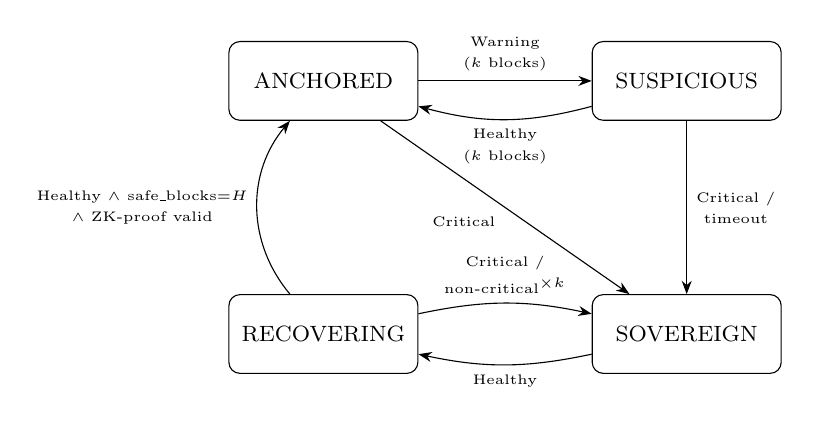
\begin{tikzpicture}[
    >=Stealth, node distance=2.2cm, auto,
    state/.style={rectangle, rounded corners, draw, minimum width=2.4cm,
                  minimum height=1cm, align=center, font=\footnotesize}
]
\node[state] (anchored) {ANCHORED};
\node[state, right=of anchored] (suspicious) {SUSPICIOUS};
\node[state, below=of suspicious] (sovereign) {SOVEREIGN};
\node[state, below=of anchored] (recovering) {RECOVERING};

\draw[->] (anchored) -- node[font=\tiny]{\shortstack{Warning\\($k$ blocks)}} (suspicious);
\draw[->] (anchored) -- node[font=\tiny, swap]{Critical} (sovereign);
\draw[->] (suspicious) -- node[font=\tiny]{\shortstack{Critical /\\timeout}} (sovereign);
\draw[->] (suspicious) to[bend left=15] node[font=\tiny]{\shortstack{Healthy\\($k$ blocks)}} (anchored);
\draw[->] (sovereign) to[bend left=12] node[font=\tiny]{Healthy} (recovering);
\draw[->] (recovering) to[bend left=12] node[font=\tiny]{\shortstack{Critical /\\non-critical$^{\times k}$}} (sovereign);
\draw[->] (recovering) to[bend left=40] node[font=\tiny]{\shortstack{Healthy $\wedge$ safe\_blocks=$H$\\$\wedge$ ZK-proof valid}} (anchored);
\end{tikzpicture}
\vspace{4mm}
\caption{Engram FSM state transition diagram. Every edge into
\textsc{Anchored} or out of \textsc{Suspicious}/\textsc{Recovering} is gated
by a hysteresis counter requiring $k$ (or $H$, the recovery-edge
hysteresis wait) consecutive blocks, not a single reading.}
\label{fig:fsm}
\end{figure}

\subsection{Network Sensors}
\label{subsec:sensors}

Three sensor categories feed the transition function; all are deterministic
so that every honest validator computes the same target state from the same
committed data.

\textbf{Bitcoin finality gap.} $\Delta H_{\text{BTC}} = H_{\text{current}} -
\min(H_{\text{submitted}}, H_{\text{anchored}})$ measures how far the latest
checkpoint is from Bitcoin confirmation. A growing gap indicates Bitcoin
congestion or a liveness attack on checkpointing. Because a delay-only metric
cannot detect a \emph{forged} checkpoint, each validator additionally
performs an off-band SPV check (Merkle-proof inclusion and block-header
verification); a failed SPV check is treated as critical-severity, on par
with an excessive gap, since it means the anchor height is unverifiable
rather than merely stale.

\textbf{Data availability gap.} $\Delta H_{\text{DA}} = H_{\text{local}} -
H_{\text{verified}}$ measures the lag between the current chain head and the
highest block for which a verified DA commitment has been received. The
target design backs this with Celestia-style data-availability sampling and
Blobstream attestation (Celestia's proof-of-inclusion bridge to external
chains); Section~\ref{subsec:sim-to-real} discusses the gap
between that target design and the current prototype, in which each
validator trusts only its own network's Celestia bridge rather than
sampling across the other validators' independent bridges.

\textbf{P2P health (tri-interface profiler).} A raw peer count cannot
distinguish a long-lived honest peer from a freshly injected Sybil, and
eclipse attacks combine several attack vectors that no single metric
captures~\cite{rehman2025eclipse}. Engram's P2P health check instead
combines six structural, behavioral, and temporal bounds -- subnet
diversity, active-anchor-peer count, clean-peer count, peer churn rate,
average peer tenure, and peer latency -- applied uniformly to the Engram
P2P interface, the Bitcoin SPV client, and the Celestia light client.
Section~\ref{subsec:rq1} and Section~\ref{subsec:limitations}
discuss the empirical effectiveness and the acknowledged scope limits of
this profiler, respectively.

\subsection{State Transition Logic and Hysteresis}
\label{subsec:transitions}

A \emph{warning} condition (a suspicious Bitcoin gap, an unhealthy DA
reading, or unhealthy P2P quality) demotes \textsc{Anchored} to
\textsc{Suspicious} only after a sustained streak of consecutive unhealthy
blocks, absorbing single-block noise. A \emph{critical} condition (an
excessive Bitcoin gap, a failed SPV check, complete anchor-peer isolation, or
a suspicious-state timeout) escalates directly to \textsc{Sovereign} from
either \textsc{Anchored} or \textsc{Suspicious}. Recovery in the opposite
direction is deliberately harder than escalation: exiting
\textsc{Suspicious} back to \textsc{Anchored}, or exiting
\textsc{Recovering} back to \textsc{Anchored}, each requires a sustained
streak of healthy blocks under a dedicated hysteresis counter, not a single
healthy reading. This asymmetry -- fast to degrade, slow and quorum-gated to
recover -- is what Section~\ref{subsec:rq3} evaluates
quantitatively across all three hysteresis-gated edges. Separately from
this hysteresis mechanism, \textsc{Suspicious} also caps the rate at which
would-be-censored transactions can be force-included, via a bounded
admission queue rather than by touching withdrawals (which stay permitted
throughout \textsc{Suspicious}, Table~\ref{tab:fsm-states}); this queue cap
is what gives \textsc{Suspicious} its ``Restricted'' throughput entry in
Table~\ref{tab:fsm-states}, and Section~\ref{sec:discussion} returns to it
as a partial mitigation against a repeated-trigger attack on the
\textsc{Anchored}$\leftrightarrow$\textsc{Suspicious} boundary.

\subsection{Extended Proposal and Consensus Protocol}
\label{subsec:proposal}

The base consensus proposal is extended with four additional fields: the
target FSM state, a DA receipt (last DA-verified height and an attestation
flag), a Bitcoin receipt (checkpoint height and canonical block hash), and a
reference to a re-anchoring ZK proof when applicable. A validator casts a
prevote for a proposal only if all of the following hold: the embedded FSM
state matches its own local transition function; the embedded health flag
matches its own aggregated health certificate; the DA receipt and Bitcoin
receipt are internally consistent and within a round-adaptive tolerance
whenever the state is \textsc{Anchored}/\textsc{Recovering} or the
corresponding layer is currently healthy; and, when the proposal claims
exit from \textsc{Recovering} to \textsc{Anchored}, a valid ZK re-anchoring
proof is attached. Section~\ref{subsec:rq4} measures the resulting
proposal-size and validation-cost overhead directly.

\subsection{Re-anchoring via Zero-Knowledge Proof of Recovery}
\label{subsec:reanchoring}

When the chain exits \textsc{Sovereign} mode, re-executing every
locally-produced block on Bitcoin would be prohibitively expensive. Instead,
a single dynamic-padding circuit (Noir, proved with Barretenberg's
UltraHonk backend)~\cite{aztec_noir_barretenberg} attests to header-chain
continuity, FSM-transition legality, and withdrawal-lock adherence across
a \textsc{Sovereign} interval of up to $N_{\max}=256$ headers, at constant
cost regardless of how many of those slots are real versus padding
(Section~\ref{sec:evaluation}). We evaluated, and rejected, a true
recursive-composition alternative in the style of proof-carrying
data~\cite{bitansky2013recursive} -- aggregating many small per-header
proofs via in-circuit verification of each inner proof -- because the
in-circuit cost of verifying one inner UltraHonk proof dwarfs the cost of
directly hashing a header, making recursion 650--1,200$\times$ slower than
the dynamic-padding circuit at matched header counts in our benchmarks
(Appendix~\ref{app:backend}); recursion is a better fit for proofs that
are themselves expensive to re-verify (e.g.\ rollup batches), not cheap
per-header hashing. A \textsc{Sovereign} interval longer than
$N_{\max}$ headers is covered by a rolling sequence of dynamic-padding
proofs, each starting where the last left off, rather than by a single
proof over the whole interval -- so verification is $O(1)$ per proof, not
$O(1)$ regardless of total interval length. Verification itself happens
off-chain: every validator runs an embedded UltraHonk verifier locally, and
only a commitment to the resulting state root is anchored on Bitcoin via
the existing checkpoint mechanism (Section~\ref{subsec:sensors}) -- Bitcoin
itself cannot evaluate the proof (its script is not expressive enough for
UltraHonk verification), so its role after re-anchoring is timestamping
and settlement of that commitment, not independent proof verification. A
full backend comparison against an alternative STARK-based prover
(Plonky3) is deferred to Appendix~\ref{app:backend}, since it evaluates a
secondary design question (prover backend choice) rather than a core
contribution.
\section{Formal Verification}
\label{sec:formal}

\subsection{Methodology: Refinement Mapping}

Directly model-checking the full system -- consensus, FSM, and network
sensors together -- is intractable at any useful scale. We instead specify a
layered hierarchy in TLA+~\cite{lamport2002specifying}: an abstract
consensus layer, a Tendermint-style consensus layer, an FSM layer, and a
server layer that composes them, and state that each concrete layer refines
the one above it. Liveness verification is reduced to a safety obligation on
a single linking invariant, \emph{QuorumOverlap} -- any two valid quorums
share at least one honest node -- following the LiDO framework's technique
for linearizable Byzantine distributed objects~\cite{qiu2024lido}, which
also requires the standard weak-fairness assumption on message delivery
after the partial-synchrony bound -- QuorumOverlap alone is a safety
invariant and does not by itself establish liveness without that fairness
assumption. The property this methodology targets is: under partial synchrony and an
$f$-bounded adversary, no two honest nodes ever decide conflicting blocks or
conflicting FSM states, and any safety violation implies the existence of
cryptographic double-signing evidence, provided (i) the health-aggregation
step is well-formed and quorum-certified, (ii) Bitcoin reorganizations are
no deeper than a configurable finality depth $K_{\text{DEEP\_FINALITY}}$,
and (iii) validators' peripheral-health views converge within the
partial-synchrony bound rather than being identical at every instant.
\textbf{We distinguish two levels of computer-checked evidence for this
property.} First, each layer's own local safety/liveness properties are
model-checked in isolation (Table~\ref{tab:formal-verification}); this
confirms each layer is internally free of the violations checked for,
within its own bounded configuration. Second, the refinement obligation
itself -- that the concrete, composed four-layer system actually simulates
the abstract layer above it, which is what would let the property transfer
from the abstract model to the concrete implementation -- is specified as
three configurations of increasing scale (C1: $N{=}4,f{=}1$; C2: deeper
consensus rounds at the same scale; C3: $N{=}7,f{=}2$) but \textbf{has not
reached convergence at any of the three scales, including the smallest
(C1), after a substantial run}. We do not report a completion estimate:
explicit-state model checking of a four-layer composition is subject to
combinatorial state-space growth, and an in-process run of this class of
check has continued well past $10^{8}$ generated states with no
discernible trend toward closure, on hardware modest enough that we cannot
responsibly project whether more compute would converge it in hours, days,
or not at all. We treat this as an open verification problem rather than a
pending task with a known cost, and return to it in
Section~\ref{sec:conclusion}. Table~\ref{tab:formal-verification}'s
per-layer results are therefore necessary but not yet sufficient evidence
for the property as stated; we report this distinction explicitly rather
than let the per-layer numbers stand in for the refinement result.

\subsection{Safety Invariants and Attack Resilience Lemmas}
\label{subsec:formal-invariants}

Five state invariants are specified and model-checked: \emph{Circuit Breaker
Isolation} (withdrawals are locked if and only if the FSM is in
\textsc{Sovereign} or \textsc{Recovering}); \emph{Hysteresis Integrity} (an
exit from \textsc{Recovering} to \textsc{Anchored} requires both the full
hysteresis wait and a valid re-anchoring proof); \emph{Suspicious-Exit
Hysteresis Integrity} (the symmetric guard on the
\textsc{Suspicious}$\to$\textsc{Anchored} edge); \emph{Strict FSM Transition
Safety} (only adjacent-state transitions are ever legal); and
\emph{Monotonicity Safety} (chain heights and time never move backward).
Beyond these state invariants, five attack-specific lemmas are enforced at
the proposal-validation layer: resistance to data withholding, resistance to
long-range/forged-anchor attacks via strict SPV verification, a
deterministic bound on Byzantine message flooding, resilience to eclipse
attacks via the six-bound P2P health check
(Section~\ref{subsec:sensors}), and accountability -- any safety violation
is designed to imply the existence of cryptographic double-signing evidence,
matching CometBFT's own equivocation evidence pool rather than requiring
custom slashing cryptography -- an accountability property inherited from
that evidence pool, not independently re-proven here.

Two threat-model boundaries -- restated here because they are direct
preconditions of the invariants above, not new assumptions -- are the
Bitcoin reorg-depth bound and the peripheral-view convergence assumption
introduced in Section~\ref{subsec:threat-model}.

\subsection{Verification Stress Test and Ablation Study}

\begin{table}[h]
\caption{Per-Layer, Non-Refinement Verification Results (TLC)}
\label{tab:formal-verification}
\centering
\footnotesize
\begin{tabular}{@{}lrrrr@{}}
\toprule
\textbf{Layer / property} & \textbf{States gen.} & \textbf{Distinct} & \textbf{Depth} & \textbf{Viol.} \\
\midrule
Tendermint (safety) & 3{,}573{,}347 & 509{,}883 & 25 & 0 \\
FSM (safety) & 1{,}022{,}325{,}986 & 3{,}386{,}761 & 22 & 0 \\
FSM (liveness) & 10{,}321{,}121 & 17{,}857 & 22 & 0 \\
\bottomrule
\end{tabular}
\end{table}

Table~\ref{tab:formal-verification} reports \emph{per-layer} model-checking
results -- each layer's own safety/liveness driver
run standalone, independent of the cross-layer refinement obligation
discussed above -- using each layer's own checked-in configuration
($N{=}4$, $f{=}1$ for Tendermint; a suspicious-state threshold of 2,
a sovereign-state threshold of 4, a hysteresis wait of 2 blocks, and a
down-hysteresis threshold of 2 for the FSM layer). All three runs
found zero violations across their explored, bounded state space. We note
this covers two of the four architectural layers described above (the
Tendermint-style and FSM layers); the abstract consensus layer and the
composing server layer do not have independent per-layer results of their
own outside the still-open refinement obligation below. As stated
above, this is evidence that each layer is individually well-behaved in
isolation; it does not by itself establish that the composed system
refines the abstract specification, which is what the still-open C1/C2/C3
sweep would show, for the reasons -- and with the same uncertainty about
cost and timeline -- discussed above; we report this honestly as an open
problem (Section~\ref{sec:conclusion}) rather than presenting the per-layer
numbers as a substitute.

The ablation study below spans two layers, not one: the circuit breaker,
hysteresis, and P2P health gate are FSM-layer mechanisms (the same scope
as the FSM rows in Table~\ref{tab:formal-verification}), while DA
consistency and the $f{+}1$ fast-forward are proposal-validation/consensus-layer
mechanisms. We state this explicitly because a mechanism's necessity is
shown only within its own layer's bounded configuration, not against the
full, composed system, until the refinement sweep above completes.

\begin{table}[h]
\caption{Ablation Study: Removing One Mechanism at a Time}
\label{tab:ablation}
\centering
\footnotesize
\begin{tabular}{@{}p{0.24\linewidth}p{0.24\linewidth}p{0.1\linewidth}p{0.24\linewidth}@{}}
\toprule
\textbf{Removed} & \textbf{Targeted threat} & \textbf{Depth} & \textbf{Violated property} \\
\midrule
Circuit breaker & Withdrawal leakage & 2 & \texttt{Sanity\_NeverAttempt} \texttt{WithdrawalLeakage} \\
Hysteresis & Premature re-anchoring & 6 & \texttt{Sanity\_NoIllegal} \texttt{HysteresisExit} \\
P2P health gate & False recovery under eclipse & 3 & \texttt{Sanity\_NoIllegal} \texttt{P2PRecovery} \\
DA consistency & Data withholding & 2 & \texttt{Sanity\_Never} \texttt{ProposeWithheldData} \\
$f{+}1$ fast-forward & Liveness deadlock & 4 & \texttt{EventualDecision} \texttt{UnderGSTLiveness} \\
\bottomrule
\end{tabular}
\end{table}

Table~\ref{tab:ablation} reports the ablation study: each row removes
exactly one defensive mechanism from the specification and re-runs
verification, expecting -- and finding -- a violation of a corresponding
sanity property. Four of five ablations were checked with Apalache's bounded
SMT search (each violation found within 25--120 seconds at a shallow depth
of 2--6), which explores depth-by-depth and is markedly faster than TLC's
breadth-first search for finding a shallow counterexample; the $f{+}1$
fast-forward ablation is liveness-only and was checked with TLC. Every
ablation reproduced a distinct, previously predicted failure mode with no
false negatives, which is the central evidence that each mechanism is
individually necessary to prevent the specific attack that motivated it
-- though single-factor ablation does not test interaction effects between
two or more mechanisms removed jointly, so this is evidence of individual
necessity, not evidence of joint sufficiency: removing the circuit
breaker permits exactly the withdrawal-leakage attack it exists to prevent;
removing hysteresis permits premature re-anchoring; removing the P2P health
gate permits an eclipsed node to force an illegal recovery; removing DA
consistency permits a data-withholding proposal to be accepted; and removing
the $f{+}1$ timeout fast-forward reintroduces a liveness deadlock under
Byzantine timeout manipulation.
\section{Experimental Setup}
\label{sec:setup}

\subsection{Testbed}

Most live results reported in Section~\ref{sec:evaluation} run on one
7-validator testbed: a genuine Cosmos SDK application on a forked CometBFT
core, deployed as a set of interconnected containers rather than an
in-process simulation. Two experiments are an explicit exception, carried
over from an earlier 4-validator cluster and not yet re-run at 7-validator
scale: the RQ1 malicious-proposer test (Section~\ref{sec:evaluation}) and
the eclipse/Sybil rows of Appendix~\ref{app:attacks}; we flag this
inconsistency rather than let the blanket ``7-validator'' framing elsewhere
in this section imply otherwise. The 7-validator testbed includes a
Bitcoin regtest network (two nodes, with a continuous mining loop producing
a block roughly every 20 seconds), a Celestia data-availability network
with seven independent bridge nodes -- one per validator, so each
validator retrieves its own DA view rather than the network sharing a
single bridge -- and a zero-knowledge prover (Noir, proved with
Barretenberg) that monitors for a \textsc{Sovereign}-mode backlog and
submits recovery-proof transactions once one accumulates. Validator gossip
runs over a dedicated full mesh of pairwise links, separate from the
network carrying Bitcoin, Celestia, and RPC traffic.

\subsection{Fault Injection}

Two classes of fault injection are used. Network-level faults are induced
through kernel-level traffic control, covering profiles for uniform
delay/jitter, packet loss, single-node isolation (an eclipse-style
partition), and heterogeneous per-validator wide-area-network delay/loss
intended to approximate seven geographically distinct regions.
Application-level faults are used where network delay alone cannot
reproduce the failure mechanism of interest: Bitcoin congestion is induced
by suspending new checkpoint submission at the application layer, so the
finality gap grows directly rather than through added RPC latency; DA
outages are induced by taking one or all seven Celestia bridge nodes
offline; and Byzantine behavior is induced either through dedicated
non-validator attacker processes or by configuring a validator instance to
misreport its proposals, double-sign, or flood the network with timeout
messages.

\subsection{Sim-to-Real Gap}
\label{subsec:sim-to-real}

This testbed approximates a real decentralized deployment; it is not one,
and we state the gap explicitly rather than leave it implicit. First, all
containers share a single physical machine's CPU and memory, so a
resource-contention condition can affect every validator simultaneously in
a way that geographically separate hardware would not; during evaluation
this manifested once as a contention-induced delay in the anchor
verification path, which we identified and corrected before the
measurements reported here were collected. Second, the testbed's Bitcoin
network produces blocks roughly 30$\times$ faster than Bitcoin mainnet;
height-based thresholds remain valid at any timescale, but the wall-clock
timings reported in Section~\ref{sec:evaluation} would be proportionally
longer in a mainnet deployment. Third, while the network runs seven
independent bridge nodes (one per validator, not a single shared bridge),
each validator's data-availability check currently trusts only its own
bridge rather than cross-validating against the other validators' bridges
through genuine light-client sampling; this is a deliberate scope choice
for the current prototype, and it means our DA-outage results measure a
bridge -- or all seven, taken offline together -- going down, not a
sampling-detected partial failure of an otherwise-healthy network. We
return to the implications of all three points in
Section~\ref{sec:discussion}.

\subsection{Baselines}

Three baselines are used across the experiments in
Section~\ref{sec:evaluation} and Appendix~\ref{app:attacks}: a vanilla
CometBFT deployment that never activates the FSM's health-aware hook and
therefore cannot leave its genesis \textsc{Anchored} state regardless of
real peripheral health, used to establish that the fallback behavior is
not an artifact of measurement; a peer-count-only P2P detector, used to
isolate the marginal benefit of the tri-interface profiler
(Section~\ref{subsec:sensors}); and each hysteresis edge's own floor
parameter value (a threshold of zero, disabling that edge's hysteresis),
used to isolate the marginal benefit of hysteresis itself.
\section{Evaluation}
\label{sec:evaluation}

To keep the main-body evaluation focused,
we report the load-bearing live experiments for each research question --
the malicious-proposer attack and the P2P quorum-gate result for RQ1, the
composite-fault stress test and the seven-scenario fault-injection sweep
for RQ2, the hysteresis parameter sweep for RQ3, and the extended-proposal
overhead benchmark for RQ4 -- out of a ten-experiment suite. The remaining
attack scenarios and a secondary ZK-backend comparison are reported in
Appendix~\ref{app:attacks} and Appendix~\ref{app:backend}; a Bitcoin-reorg
boundary test is reported in Appendix~\ref{app:reorg}. Unless noted
otherwise, every number below is a live measurement on the real 7-validator
testbed (Section~\ref{sec:setup}), not an in-process simulation; the
malicious-proposer test below is the one exception, run at 4-node scale as
disclosed in Section~\ref{sec:setup}.

\label{subsec:rq1}

\textbf{Malicious proposer.} We selected the malicious-proposer scenario as
our first representative attack because it directly exercises the extended
proposal's core safety property: a Byzantine leader that fabricates its
FSM-state claim. In this scenario, a compromised validator (25\% of voting
power at 4-node scale) is configured to broadcast a proposal whose FSM-state
field does not match its own honest sensor readings. Across
the live run, \textbf{safety held with zero AppHash divergence}: every
honest validator's independent re-evaluation of the FSM's own transition
function rejected the forged claim at the
proposal-validation step, consistent with the \emph{Strict FSM Transition
Safety} and \emph{Accountability} properties verified in
Section~\ref{sec:formal}. This result is one row of a broader ten-scenario
attack suite covering eclipse, Sybil, data withholding, forged Bitcoin
receipts, withdrawal-during-\textsc{Sovereign}, censorship, a combined
attack, double-signing, and timeout flooding, all of which held safety with
zero divergence; the full per-attack results are reported in
Appendix~\ref{app:attacks}.

\textbf{P2P quorum gate.} Our second RQ1 result addresses a different
safety property: does the tri-interface P2P profiler (Section~\ref{subsec:sensors})
translate into a real consensus safeguard, or only a monitoring signal? We
compare it against a peer-count-only baseline across four synthetic attacks
via a 2{,}000-trial-per-cell Monte Carlo study, then confirm the two most
diagnostic attacks live on the real cluster.

\begin{table}[h]
\caption{P2P Detector Accuracy: Tri-Interface vs.\ Peer-Count-Only (Synthetic, 2{,}000 trials/cell)}
\label{tab:p2p-detector}
\centering
\footnotesize
\begin{tabular}{@{}lrr@{}}
\toprule
\textbf{Attack} & \textbf{Detection delay (snapshots)} & \textbf{Evasion threshold} \\
\midrule
P1 Peer-slot exhaustion & 2.23 & 0.17 \\
P2 Multi-subnet Sybil & 1.00 & 0.00 \\
P3 Churn-based rotation & 1.70 & 0.12 \\
P4 Relay-node latency & 2.71 & 0.25 \\
\bottomrule
\end{tabular}
\\[2pt]
\footnotesize Peer-count-only baseline: 100\% false-negative rate and an
evasion threshold of 1.0 (never caught, at any intensity) on all four
attacks, by construction -- all four preserve clean-peer count. The
tri-interface profiler holds 0\% false positives and 0\% false negatives on
every attack.
\end{table}

Table~\ref{tab:p2p-detector} shows the tri-interface profiler catches every
attack a peer-count-only detector is structurally blind to, across the full
range of intensities an adaptive adversary could search (evasion threshold
$\leq 0.25$ in every case), and this advantage is stable across three
different attack-ramp shapes (linear, front-loaded, stealthy-slow; 300/300
trials caught in every shape$\times$attack cell) and independent of
concurrent Bitcoin/DA degradation. Live confirmation isolates a subtler
finding than raw detection accuracy: a real quorum gate on top of that
detection. Attack P3 (churn-based rotation, eight repeated container
restart cycles on 2 of 7 proposers, $\sim$29\% of voting power)
is correctly \emph{sensed} -- the peer-churn-rate metric on both attacked nodes
crosses the detection threshold -- yet produces \textbf{no committed FSM
transition}, because a transition requires $\geq 2f{+}1$ voting
power's signed observations before it commits, and a
minority-visible degradation cannot supply that quorum. Attack P4
(sustained 350$\pm$50\,ms delay on all of one validator's real P2P
interfaces, visible to 7 of 7 validators, i.e.\ full quorum) produces the
opposite outcome: a full, correctly-bounded
\textsc{Anchored}$\to$\textsc{Suspicious}$\to$\textsc{Sovereign} cascade
(+39\,s, +72\,s relative to the attack start) that holds for the entire
244-second attack window and recovers
(\textsc{Recovering}$\to$\textsc{Anchored}) within 5 seconds of the delay
clearing, as shown in Fig.~\ref{fig:a4-cascade}.

\begin{figure}[h]
\centering
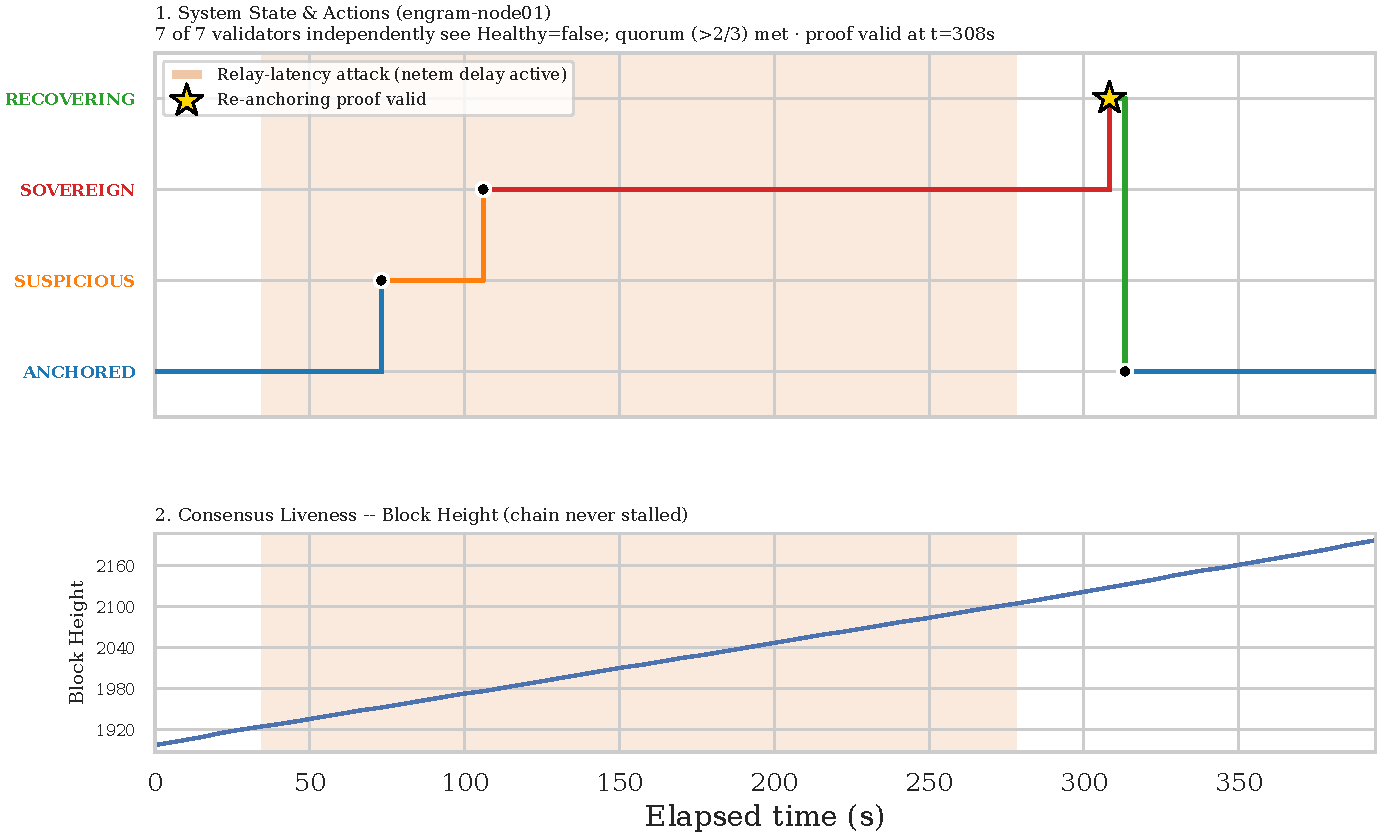
\includegraphics[trim=0 0 0 38pt, clip, width=\linewidth]{figures/figure5_a4_cascade_timeline_live.pdf}
\caption{FSM cascade under a real, quorum-visible P2P relay-latency attack
(P4): all 7 validators independently sense the degradation, the transition
commits once quorum is met, and block production (bottom panel) never
stalls through the cascade or the recovery.}
\label{fig:a4-cascade}
\end{figure}

Together, P3 and P4 are two outcomes of one mechanism, not two separate
detector results: the identical class of real, sensor-confirmed P2P
degradation is correctly blocked from committing when only a minority of
validators observes it, and correctly drives a bounded, liveness-preserving
state cascade when a supermajority does. This is a specific instance of the
safety property RQ1 asks for -- resistance to a Byzantine-influenced
minority forcing an unwarranted state transition -- though we note it
exercises the quorum-threshold mechanism under adversarial network
conditions rather than the forged-receipt or data-withholding vectors RQ1
also names; those are addressed separately by the malicious-proposer result
above and by Appendix~\ref{app:attacks}'s broader attack suite.

\label{subsec:rq2}

\textbf{Composite fault.} To answer RQ2 we first ran a single, continuous,
scripted composite-fault sequence rather than isolated single-fault
scenarios: growing Bitcoin congestion, layered onto a full Celestia DA
outage (all seven independent bridges stopped together), layered onto three
cycles of packet loss on the validator P2P network, all three overlapping
at their peak, followed by a sequential, real recovery -- run under a
standing wide-area-network latency baseline. Fig.~\ref{fig:fsm-timeline}
plots the resulting FSM state timeline.

\begin{figure}[h]
\centering
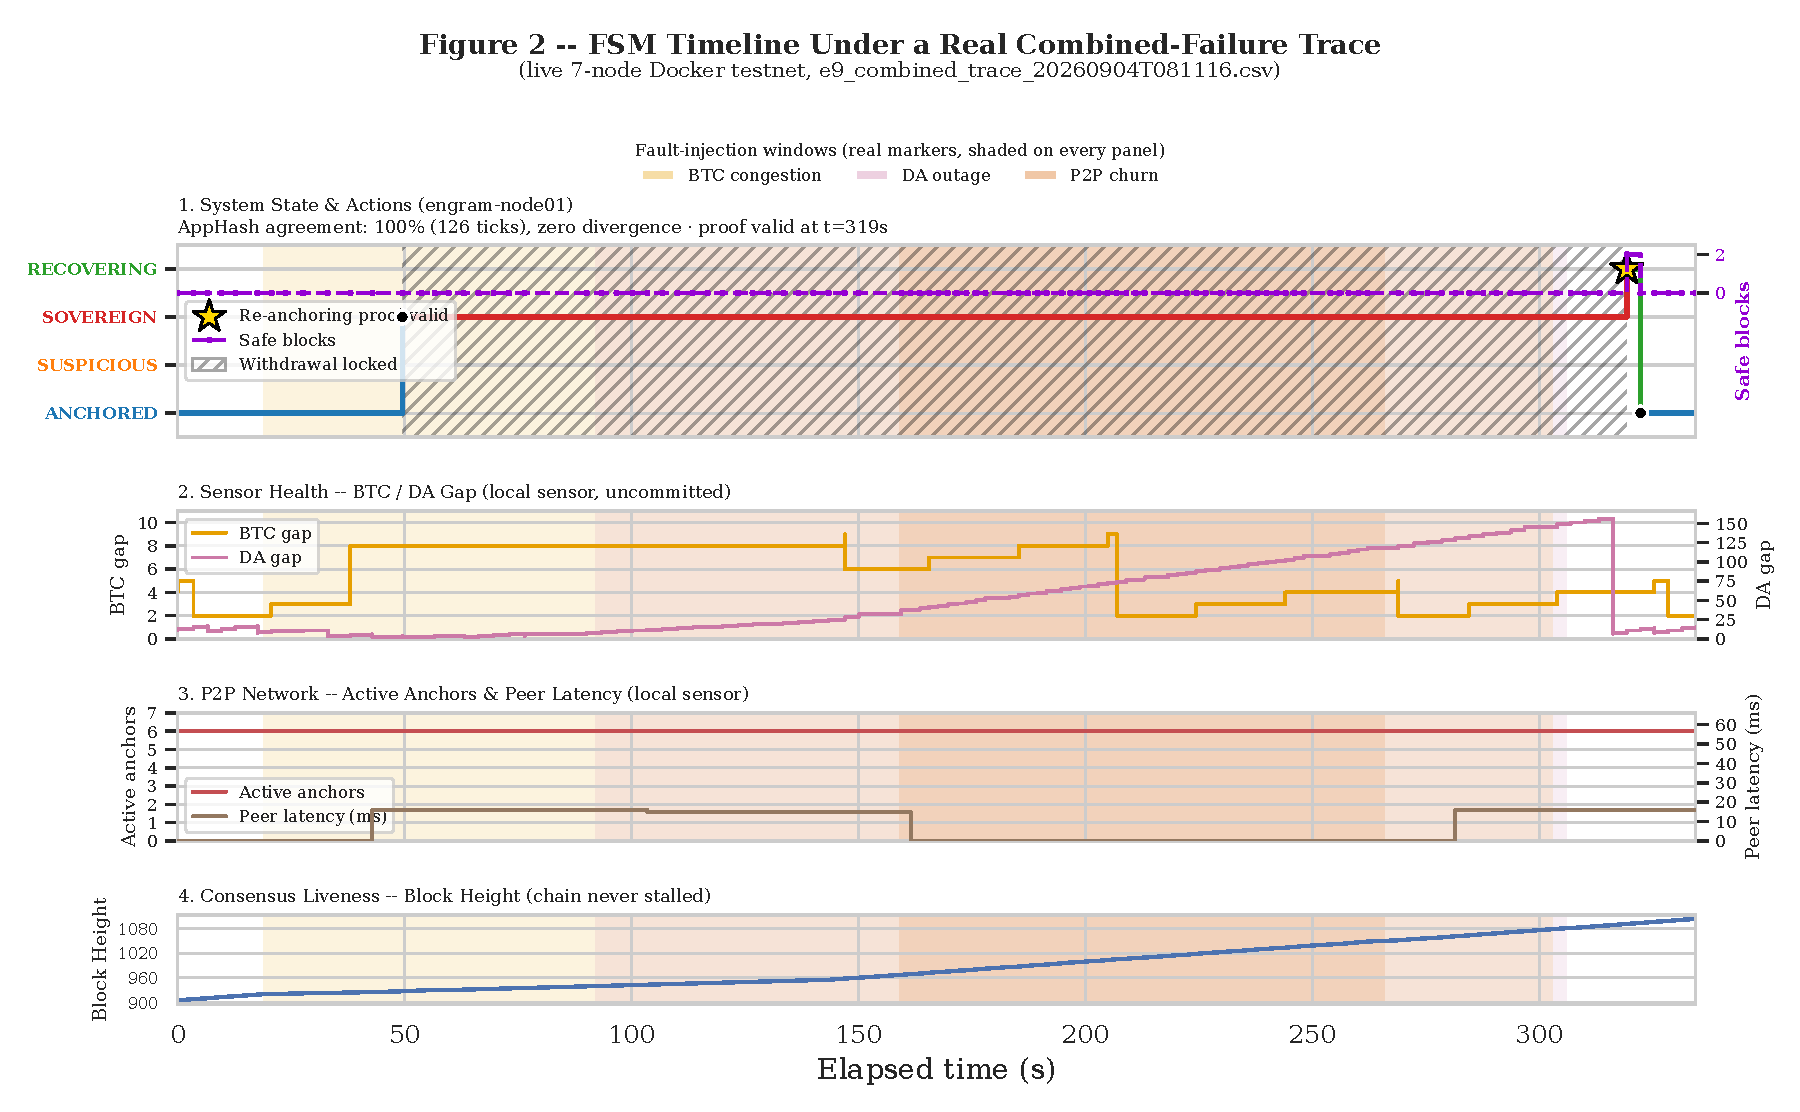
\includegraphics[trim=0 0 0 40pt, clip, width=0.95\linewidth]{figures/figure2_trace_timeline_live.pdf}
\caption{FSM state timeline, sensor readings, P2P network state, and block
height under a layered composite fault sequence (Bitcoin congestion + DA
outage + P2P churn, overlapping at their peak).}
\label{fig:fsm-timeline}
\end{figure}

Over a 341-second run (742 samples, 126 polling ticks), the chain height
progressed continuously from 905 to over 1093 with \textbf{no stalled
round}, and all seven validators reached \textbf{100\% AppHash agreement}
across every tick, with zero divergent heights and zero RPC errors. The
chain reached \textsc{Sovereign} under the combined fault, then completed a
real recovery cycle -- \textsc{Recovering} at $t{=}321$\,s,
\textsc{Anchored} at $t{=}324$\,s -- once the injected faults were healed.
Withdrawals were locked for the entire \textsc{Sovereign}/\textsc{Recovering}
window and unlocked only after the transition back to \textsc{Anchored},
matching the circuit-breaker invariant of Section~\ref{sec:formal}; the
re-anchoring proof (Section~\ref{subsec:reanchoring}) was confirmed valid at
$t{=}319$\,s, ahead of the state transition it gates.

\textbf{Seven-scenario fault-injection sweep.} The composite trace shows
the mechanism survives worst-case overlap, but does not isolate which
failure mode drives which behavior. We complement it with a longer,
864-second live run walking the chain through seven sequential scenarios --
S1 normal baseline, S2 Bitcoin congestion, S3 DA outage, S4 partial P2P
eclipse, S5 total anchor isolation, S6 combined Bitcoin+DA failure, and S7
recovery -- each building on the last, with 153 real FSM transitions logged
across all 7 validators. Fig.~\ref{fig:s1-s7} plots the full continuous
timeline.

\begin{figure}[h]
\centering
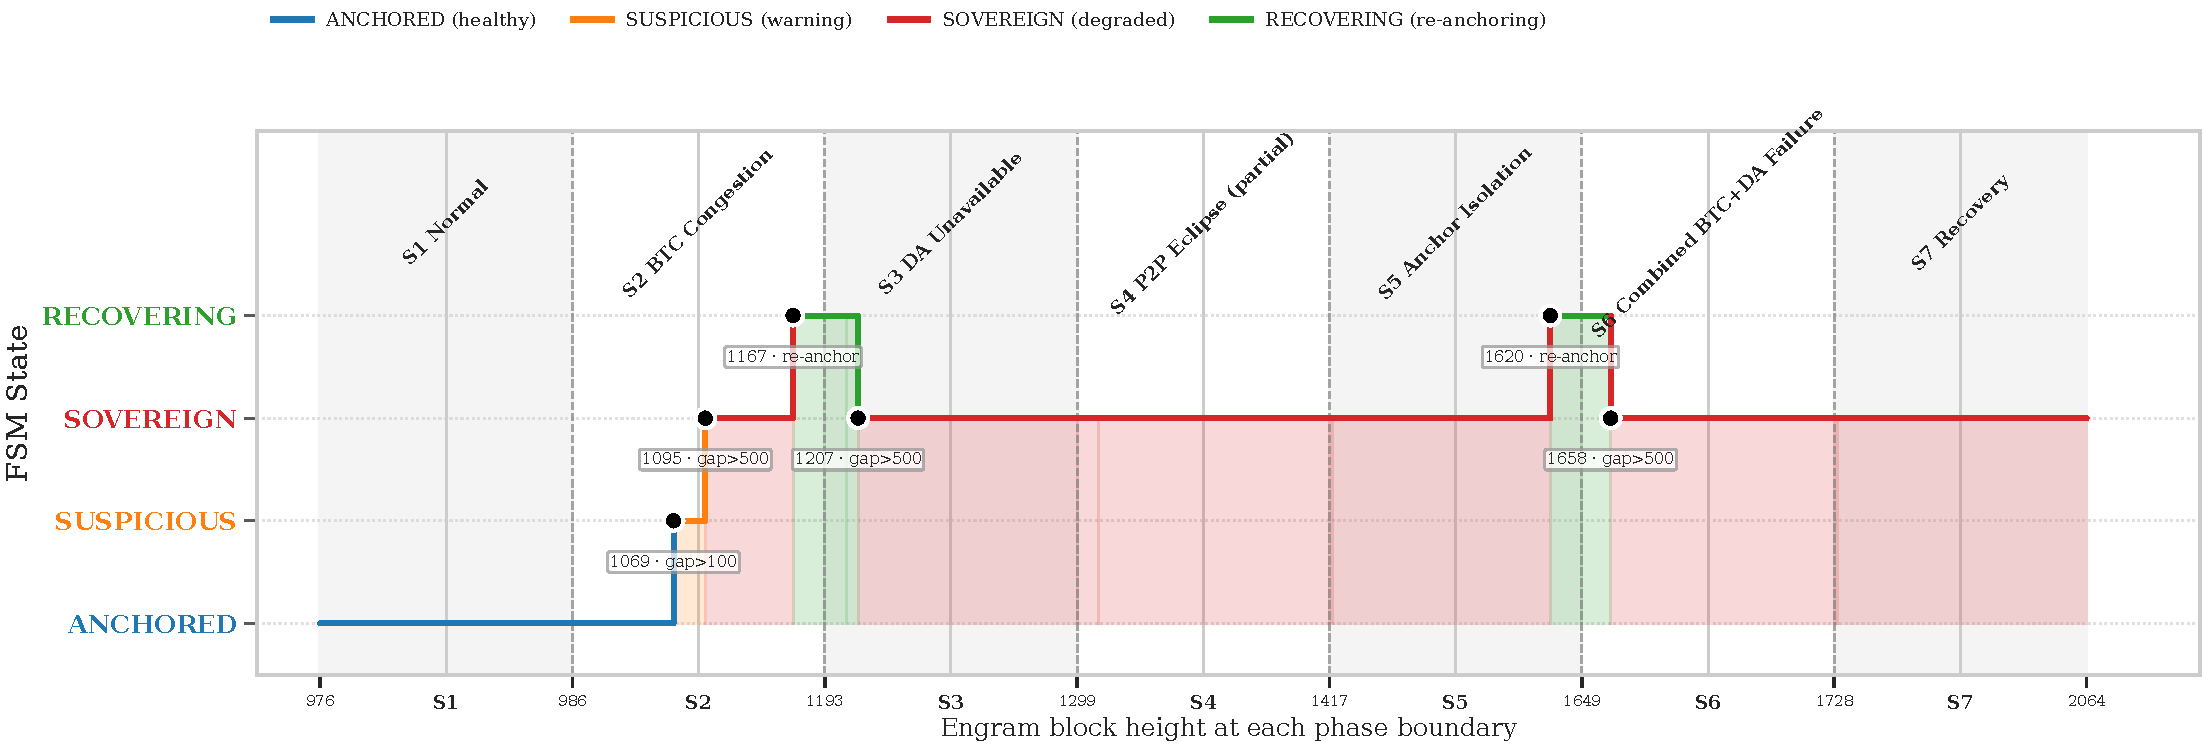
\includegraphics[trim=0 0 0 22pt, clip, width=0.95\linewidth]{figures/figure3_single_timeline_live.pdf}
\caption{Continuous FSM-state timeline across seven sequential
fault-injection scenarios (S1--S7), true block-height ranges, live
7-validator testbed. Each scenario begins where the previous scenario's
recovery ended.}
\label{fig:s1-s7}
\end{figure}

Every scenario shows the correct qualitative response: S2 (Bitcoin
congestion) and S3 (DA outage) each independently escalate through
\textsc{Suspicious} to \textsc{Sovereign} and recover; S4 (partial P2P
eclipse) escalates fully to \textsc{Sovereign}, while S5 (total anchor
isolation on one of seven validators) only ever produces a transient,
hysteresis-absorbed \textsc{Suspicious} dip that self-heals, because losing
1 of 7 anchor peers does not zero out the active-anchor-peer count and therefore
never satisfies the immediate-escalation condition -- a direct, live
confirmation that S4 and S5 are qualitatively different failure classes, not
two instances of the same detector saturating; S6 (Bitcoin and DA failing
together) escalates directly to \textsc{Sovereign}; and S7 (recovery) closes
the loop back to \textsc{Anchored} via a real submitted re-anchoring proof.
Two results from this run are worth highlighting beyond the qualitative
pattern. First, S2 itself shows two brief, real \textsc{Suspicious} blips
(19--22\,s and 77--80\,s into the scenario) that hysteresis absorbs back to
\textsc{Anchored} before the scenario's real escalation at 141\,s -- the
first confirmation on physical infrastructure that hysteresis absorbs
genuine noise, a
property previously shown only in E5's synthetic sweeps
(Section~\ref{subsec:rq3}). Second, per-scenario throughput held
close to baseline throughout: block-interval means ranged 1.30--1.93\,s
across all seven scenarios (vs.\ 1.34\,s at the S1 healthy baseline), with
the two heaviest scenarios (S4 partial eclipse and S7 recovery) showing the
largest, but still bounded, tail latency (p95 4.27\,s and 3.10\,s
respectively). Together with the composite-fault result above, this
answers RQ2 affirmatively from two complementary angles: the chain keeps
committing blocks under both an overlapping worst-case fault and under each
individual failure mode in isolation, and recovers correctly in every case,
rather than halting.

\label{subsec:rq3}

RQ3 asks whether hysteresis prevents oscillation (``flapping'') once
peripherals recover, without unduly delaying recovery. We swept the
governing threshold on each of the three hysteresis-gated edges --
\textsc{Recovering}$\to$\textsc{Anchored},
\textsc{Anchored}$\to$\textsc{Suspicious}, and
\textsc{Suspicious}$\to$\textsc{Anchored} -- both in-process (fixed-seed
synthetic noise, for a clean monotonic baseline) and live on the real
7-validator cluster (real network noise, which does not cancel out the way
a fixed seed does). Fig.~\ref{fig:hysteresis} plots the resulting
uptime/absorption trade-off for all three edges.

\begin{figure}[h]
\centering
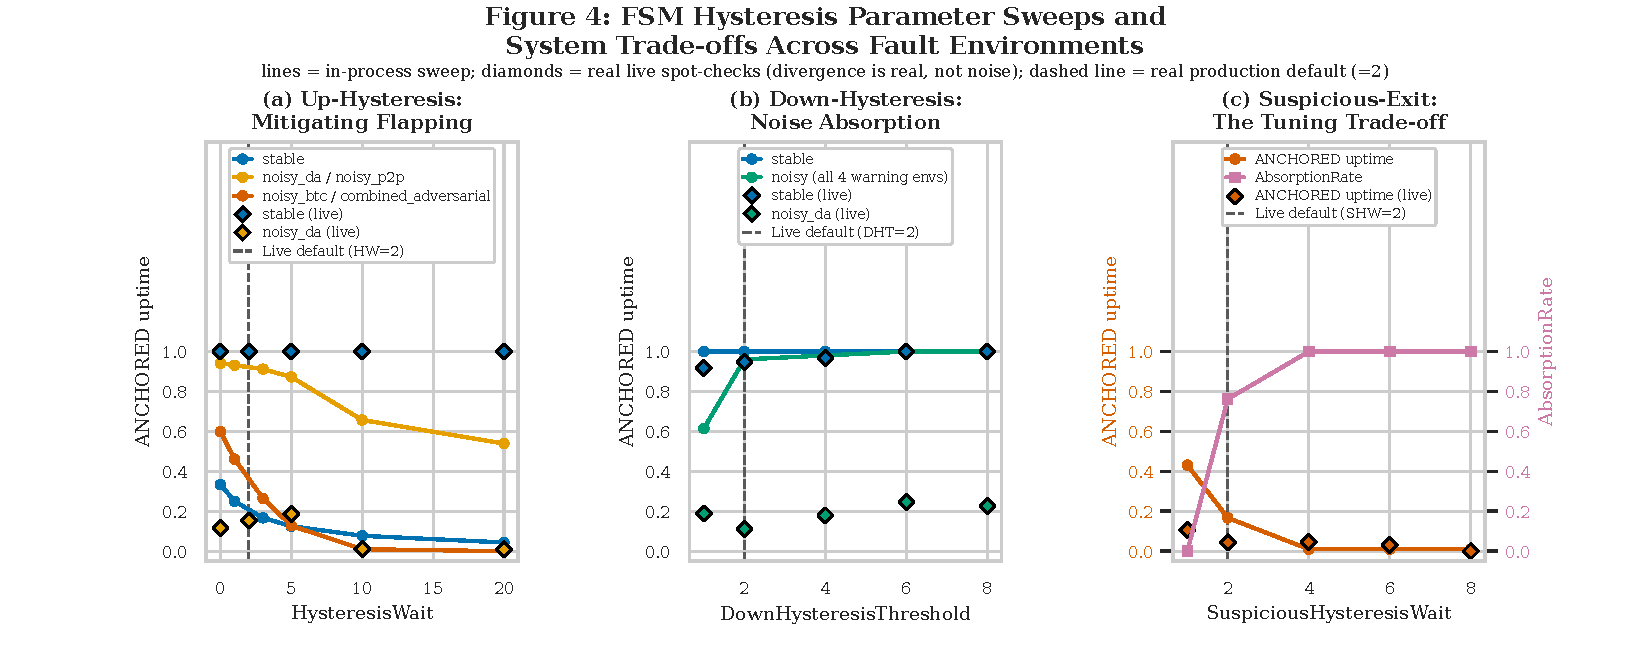
\includegraphics[trim=0 0 0 28pt, clip, width=0.95\linewidth]{figures/figure4_hysteresis_tradeoffs.pdf}
\caption{Hysteresis parameter sweep across all three absorb edges. Lines:
in-process sweep under different noise profiles; diamonds: live spot-checks
on the real 7-validator cluster (divergence from the in-process line is
real network behavior, not measurement noise); dashed line: the protocol's
live production default.}
\label{fig:hysteresis}
\end{figure}

\begin{table}[h]
\caption{Down-Hysteresis Sweep (\textsc{Anchored}$\to$\textsc{Suspicious}),
In-Process}
\label{tab:hysteresis-down}
\centering
\footnotesize
\begin{tabular}{@{}lrrrrr@{}}
\toprule
\textbf{Threshold} & 1 & 2 & 4 & 6 & 8 \\
\midrule
Flapping (count)     & 31 & 1 & 1 & 0 & 0 \\
Anchored uptime (\%) & 61.39 & 96.04 & 98.02 & 100.00 & 100.00 \\
Absorption rate (\%) & 0.00 & 94.74 & 95.24 & 100.00 & 100.00 \\
\bottomrule
\end{tabular}
\end{table}

Table~\ref{tab:hysteresis-down} shows the clearest single result: on the
\textsc{Anchored}$\to$\textsc{Suspicious} edge, raising the down-hysteresis
threshold from 1 to 4 collapses flapping from 31 events to 1 and raises
anchored uptime from 61.4\% to 98.0\%, and the absorption rate saturates
near 100\% by threshold 4--6. The live spot-check on the real cluster
confirms this is not merely a synthetic artifact but shows a stronger,
practically important finding: under real wide-area-network jitter alone
(with \emph{no} injected fault), thresholds 1, 2, and even 4 still produced
spurious flapping, and only threshold $\geq 6$ was clean (0 flapping, 100\%
uptime) -- a materially stronger requirement than the protocol's own default
value of 2, and a concrete, actionable recommendation for deployment in a
WAN-realism regime. We flag an apparent tension we have not resolved: the
composite-fault, seven-scenario, and P4 experiments above all ran at this
same default threshold of 2 under the same WAN-jitter baseline, yet report
no comparable flapping. This is not necessarily a contradiction --
this dedicated sweep is the only experiment that explicitly counts
flapping events in isolation from any other injected fault; the other
experiments track qualitative correctness (AppHash agreement, block
production) rather than a flapping count, so an occasional spurious flap
not large enough to affect those outcomes would not have been visible in
their results either way. We report this as a difference in measurement
scope, not as evidence that the other experiments were in fact flap-free.
The symmetric edges show consistent trade-offs in the
opposite direction: on the \textsc{Recovering}$\to$\textsc{Anchored} edge, a
larger hysteresis-wait threshold strictly reduces anchored uptime under
sustained critical-level noise (59.8\%$\to$0.0\% as the threshold goes from
0 to 20) -- a designed, expected negative result, since critical-level
conditions bypass hysteresis by construction rather than being absorbed by
it. On the \textsc{Suspicious}$\to$\textsc{Anchored} edge, absorption rate
rises from 0\% to 100\% as the threshold goes from 1 to 4, but this is a
genuine trade-off, not a free improvement: the same accumulating
suspicious-state duration timer that a longer threshold is meant to
outlast can independently force escalation to \textsc{Sovereign} once it
hits its own cap, so only the smallest threshold values in our sweep
(1--2) actually reached \textsc{Anchored} within the timeout window. We
discuss the resulting open design question -- asymmetric hardening across
edges -- in Section~\ref{sec:discussion}. Appendix~\ref{app:reorg} reports a
complementary recovery-boundary result: how far a real Bitcoin
reorganization can go before the same FSM reacts at all.

\label{subsec:rq4}

\begin{table}[h]
\caption{Extended Proposal Overhead vs.\ Vanilla CometBFT}
\label{tab:overhead}
\centering
\footnotesize
\begin{tabular}{@{}lrr@{}}
\toprule
\textbf{Metric} & \textbf{Vanilla} & \textbf{Engram (extended)} \\
\midrule
Steady-state proposal tax & 0 B/block & +228 B/block \\
Full proposal-validation CPU & --- & 18{,}252 ns \\
p95 commit latency @ 20 tx/s & 1.017 s & 1.021 s \\
Blocks/s @ 20 tx/s ($n{=}5$) & 0.953 $\pm$ 0.007 & 0.743 $\pm$ 0.008 \\
Tx-accepted/s @ 20 tx/s & 20.00 $\pm$ 0.00 & 19.99 $\pm$ 0.00 \\
\bottomrule
\end{tabular}
\end{table}

Table~\ref{tab:overhead} answers RQ4 directly. On the healthy path, the
extended proposal adds a small, near-constant \textbf{+228 bytes per block}
(100\% of blocks carry the marker) versus zero for vanilla CometBFT; a live
376-block sample confirms 100\% marker coverage with per-state average
proposal sizes of 247--270 bytes, and the one recovery-proof-carrying block
observed matched the expected $\sim$14.7\,KB proof-plus-envelope size from
Section~\ref{subsec:reanchoring}. Validation CPU cost is negligible: the
full proposal-validation path costs 18{,}252\,ns (18.25\,$\mu$s) on a
steady-state, non-recovery block -- several orders of magnitude below both
CometBFT's own commit-timeout parameter (hundreds of milliseconds) and this
cluster's $\sim$1-second block interval. Under load ramped from 5 to 100
tx/s, we found \textbf{no throughput ceiling within the tested range}:
every rate stage accepted
100\% of submitted transactions in both modes, and p95 commit latency
stayed essentially flat ($\sim$1.01--1.02\,s) regardless of rate, dominated
by the block interval rather than load. At a fixed rate of 20 tx/s with
$n{=}5$ independent repeats, the extended mode's block-production rate
(0.743 $\pm$ 0.008 blocks/s) was consistently, but modestly, lower than
vanilla's (0.953 $\pm$ 0.007 blocks/s) -- a stable $\sim$23--27\% gap in
per-round overhead (Cohen's $d{=}$--25.3, a very large but tightly
reproducible effect) that a throughput-corrected metric shows converges
between the two modes, indicating the gap is round-skip overhead rather than
a growing backlog. We regard this as an acceptable, bounded cost given the
liveness and safety guarantees demonstrated under RQ1--RQ3.
\section{Discussion and Limitations}
\label{sec:discussion}

\subsection{Interpretation of Results}

Taken together, Sections~\ref{sec:formal} and~\ref{sec:evaluation} support
the paper's central claim, but with an asymmetry worth stating plainly: the
empirical evaluation runs the full, composed, real system (all layers
integrated, real Go code, real infrastructure), while the completed formal
verification is currently per-layer only -- each layer shown internally
free of violations in isolation, not yet shown to correctly refine the
abstract specification as a composed whole (Section~\ref{sec:formal}). This
means the live testbed currently carries more of the burden of demonstrating
whole-system correctness than the formal verification does; the formal side
contributes a precise statement of the target safety-and-accountability
property, machine-checked evidence at the component level, and a
five-mechanism ablation study showing each mechanism is individually
necessary at the FSM layer, while the live evaluation shows the resulting
design behaves correctly under real, not merely modeled, faults -- most
directly in the RQ2 composite-fault trace, where a real
\textsc{Sovereign}$\to$\textsc{Recovering}$\to$\textsc{Anchored} cycle
completes with 100\% AppHash agreement under three overlapping fault classes
at once. Neither result alone would be sufficient: the TLA+ model does not
capture real network timing, container resource contention, or the actual
Noir/Barretenberg proving pipeline, while the live testbed alone cannot
explore the state space exhaustively enough to guarantee the absence of
subtle safety violations, and its qualitative demonstrations (composite
fault, seven-scenario sweep, the P4 cascade, the reorg-depth reaction) are
each a single trial rather than a repeated, statistically characterized
sample -- unlike the properly repeated E5 hysteresis sweep, the E7 overhead
measurement ($n{=}5$), and the E4 synthetic Monte Carlo study (2,000
trials/cell). We report exact transition timings from these single-trial
runs (e.g.\ ``$t{=}321$\,s'') as one observed instance of correct behavior,
not as a characterized distribution. Repeating these live trials is
straightforward future work; the cross-layer refinement check discussed in
Section~\ref{sec:formal} is a separate, open-ended gap whose resolution we
cannot schedule (Section~\ref{sec:conclusion}).

\textbf{Open question: asymmetric hardening.} Our RQ3 results
(Section~\ref{sec:evaluation}) surface a genuine, unresolved design gap.
Exponential backoff exists on the \textsc{Recovering}$\to$\textsc{Sovereign}
edge specifically to defend against a cheap, repeatable attack that forces
premature demotion, but the same attack shape is available on the
\textsc{Anchored}$\leftrightarrow$\textsc{Suspicious} boundary, whose
thresholds do not grow the more they are triggered. A partial mitigation
exists at the application layer (a queue cap on forced-transaction admission
while \textsc{Suspicious}), but whether this edge needs the same backoff
hardening already applied to \textsc{Sovereign}/\textsc{Recovering} remains
open, and we flag it as a concrete direction for follow-up work
(Section~\ref{sec:conclusion}) rather than resolving it speculatively here.

\textbf{Griefing surface created by the fallback itself.} Forcing
\textsc{Sovereign} is not only a liveness question but a security
tradeoff: an adversary who degrades only a validator-visible \emph{view}
of Bitcoin, DA, or P2P health -- without compromising any validator's
keys -- can drive a supermajority-visible cascade
(Section~\ref{sec:evaluation}, P4) and lock withdrawals network-wide for
as long as the degraded view persists. We have not quantified the
attacker's cost against this benefit (e.g.\ the cost of sustaining a
network-level attack against a supermajority of validators' Bitcoin/DA/P2P
connectivity, versus the value of a network-wide withdrawal freeze to that
attacker), nor analyzed the security implication of a long-range fork
between the Bitcoin-anchored history and the sovereign history at
re-anchoring time. Both are open problems this paper's evaluation does not
resolve.

\subsection{Limitations}
\label{subsec:limitations}

Section~\ref{subsec:sim-to-real} already discloses three gaps between this
testbed and a genuinely distributed, mainnet-scale deployment: a shared
physical host, an accelerated Bitcoin timescale, and single-source-per-validator
DA trust. Rather than restate those facts, we state here what each one
means for how the results in Section~\ref{sec:evaluation} should be read,
plus three further limitations not covered there.

\textbf{Single physical host.} Because every validator, plus the Bitcoin
and Celestia networks, share one machine's resources, our measured
overhead numbers (RQ4) are a reasonable but not definitive proxy for a
genuinely distributed deployment, and our wide-area-network fault
injection, while using kernel-level traffic control, approximates rather
than reproduces true geographic distribution.

\textbf{Accelerated Bitcoin timescale.} Because the testbed's Bitcoin
network runs roughly $30\times$ faster than mainnet, readers should treat
our wall-clock timings (e.g.\ the 341-second RQ2 trace) as demonstrating
\emph{correct sequencing} of the recovery process, not as mainnet-calibrated
latency figures; height-based thresholds are unaffected.

\textbf{Single-source-per-validator DA trust.} Because each validator
trusts only its own bridge rather than sampling across the other six, our
DA-outage results should be read as measuring a bridge (or all seven
together) going down, not as a sampling-detected partial failure of an
otherwise-healthy network; closing this gap is future work
(Section~\ref{sec:conclusion}).

\textbf{Single Byzantine actor at a time.} Every live attack in this paper
-- the malicious proposer, the ten-scenario suite in
Appendix~\ref{app:attacks}, and P3/P4 -- compromises exactly one validator
or attacker container at a time. The formal threat model bounds up to $f$
simultaneously Byzantine validators ($f{=}2$ at $N{=}7$), but no live
experiment has exercised $f$ validators colluding at once (e.g.\ two
validators jointly forging a certificate or double-signing in coordination);
single-actor tests establish a safety margin, not the formally-bounded
worst case. Relatedly, the ten-attack suite tests a Byzantine
\emph{proposer} forging its proposal's FSM-state field, but does not
separately test a Byzantine validator submitting a false individual health
certificate into the health-certificate aggregation step that precedes
consensus -- a related but distinct vector we have not confirmed is
covered by an existing test.

\textbf{Near-quorum split views untested.} Section~\ref{subsec:threat-model}
notes that validators running identical thresholds can still disagree if
their own external reads of Bitcoin, DA, or P2P health genuinely differ.
Every split view we tested is decisive (a self-healing 1-of-7 view in S5,
a sub-quorum 2-of-7 view in P3), not a persistent split straddling the
$\geq 2f{+}1$ quorum boundary (e.g.\ 3-of-7 or 4-of-7), which could in
principle cause repeated nil-prevotes and round failures rather than a
clean commit either way. We note this because it offers one plausible,
unconfirmed explanation for the $\sim$23--27\% block-production-rate
reduction observed even on the fully healthy RQ4 path
(Table~\ref{tab:overhead}): we describe that gap as ``round-skip
overhead'' without having isolated whether occasional round-level
disagreement of this kind, rather than pure validation latency, is what
drives it.

\textbf{Throughput tested only up to 100 tx/s.} RQ4's ``no throughput
ceiling'' finding (Section~\ref{sec:evaluation}) holds within the tested
range; we did not search for a rate at which the extended proposal's
per-block byte overhead compounds with mempool or gossip costs into a
measurable ceiling, so readers should not read this as a claim that no such
ceiling exists at higher throughput.

Beyond these six, the two threat-model boundaries introduced in
Section~\ref{subsec:threat-model} (the Bitcoin reorg-depth bound and the
peripheral-view convergence assumption) remain conditions on, rather than
caveats against, the safety and accountability property targeted in
Section~\ref{sec:formal}; we do not restate them a third time here.

\subsection{Threats to Validity}

\textbf{Internal validity.} Sharing one physical host (above) is the primary
threat to internal validity for our cost measurements; we mitigate this by
reporting both a ramped-load sweep and a fixed-rate, $n{=}5$-repeat
measurement with confidence intervals (Section~\ref{subsec:rq4}),
which shows the measured overhead gap is stable and reproducible rather than
noise, but does not eliminate host-sharing as a contributing factor to the
absolute numbers.

\textbf{External validity.} Results at 7-validator scale, on a single
physical host, may not extrapolate linearly to mainnet-scale validator sets
or genuinely distributed infrastructure; we regard our results as
establishing correctness and a bounded-overhead \emph{trend}, not as
mainnet-calibrated performance figures.

\textbf{Construct validity.} We use AppHash agreement and divergence
counts as our operational proxy for safety, and block
height progression / commit rate as our operational proxy for liveness,
consistent with how CometBFT-family systems are conventionally evaluated;
readers should note that this proxies the properties formally verified in
Section~\ref{sec:formal} rather than independently re-deriving them.
\section{Conclusion}
\label{sec:conclusion}

We presented the Engram Hybrid Adaptive Consensus, a CometBFT-based protocol
that folds peripheral network health -- Bitcoin settlement, Celestia data
availability, and P2P quality -- into the consensus object as a first-class,
quorum-agreed variable, degrading through a four-state finite state machine
into a local fallback that keeps producing blocks without external
corroboration instead of halting when a peripheral
layer fails. We backed this design with two complementary forms of evidence.
Formally, each protocol layer's own bound-model-checked safety and liveness
properties found zero violations across 3.39 million distinct explored
states ($1.02\times10^{9}$ generated) at that layer's own checked-in scale, and a five-mechanism ablation
study at the FSM layer showed that removing any one safety mechanism
reproduces a distinct, predicted failure mode, evidence that each mechanism
is individually load-bearing at that layer; the cross-layer refinement
check that would extend this guarantee to the full composed system at
production scale is specified but not yet run to completion, and we regard
the live evaluation below as currently carrying the larger share of
whole-system evidence. Empirically, on a real 7-validator testbed (with two
exceptions run at 4-node scale, Section~\ref{sec:setup}) against live
Bitcoin and Celestia networks, the protocol (i) maintained \textbf{safety}
with zero AppHash divergence under representative Byzantine attacks, while
improving \textbf{liveness} by sustaining continuous block production and
completing a full recovery cycle under a layered composite fault; (ii)
provided \textbf{controlled recovery}, with hysteresis measurably trading
uptime against flapping resistance in a tunable way across all three
hysteresis-gated edges; and (iii) incurred \textbf{acceptable overhead} --
+228 bytes per block and $\sim$18.25\,$\mu$s of validation cost on the
healthy path, with no throughput ceiling found within the tested range (up
to 100 tx/s). Together, these results indicate that treating
peripheral-layer health as a first-class consensus variable is a practical
way to trade a small, bounded overhead for substantially stronger liveness
guarantees in modular blockchain systems, though the whole-system claim
currently rests more heavily on live evidence than on the formal side,
for reasons detailed in Section~\ref{sec:discussion}.

\subsection*{Future Work}

Eight directions follow directly from the limitations discussed in
Section~\ref{sec:discussion}. First, the cross-layer refinement
verification sweep (Section~\ref{sec:formal}) remains an open problem
rather than a scheduled task: even its smallest configuration (C1, $N{=}4$)
has not reached convergence, and given the combinatorial state-space growth
typical of explicit-state model checking over composed protocol layers, we
cannot commit to a timeline or a resource budget that would close it.
Narrowing this gap may call for a different verification strategy
altogether -- symmetry reduction, statistical model checking, or a
deductive proof in the style discussed in Section~\ref{sec:related} --
rather than simply more compute directed at the same explicit-state search.
Second, re-running the live evaluation across genuinely distributed
physical hosts, rather than one shared machine, would remove the
single-host resource-contention confound noted in
Section~\ref{subsec:limitations}. Third, closing the gap between the target
DA sampling design and the current single-bridge-per-validator prototype
(Section~\ref{subsec:sensors}) would strengthen the DA-outage results from
measuring a bridge failure to measuring a genuinely sampling-detected
partial DA failure. Fourth, the open question raised in
Section~\ref{sec:discussion} -- whether the
\textsc{Anchored}$\leftrightarrow$\textsc{Suspicious} boundary needs the
same exponential-backoff hardening already applied to the
\textsc{Sovereign}/\textsc{Recovering} edges -- remains an open design
problem for future protocol iterations. Fifth, re-running the
malicious-proposer test and the A1/A2 eclipse/Sybil scenarios at the same
7-node scale used elsewhere would remove the scale inconsistency noted in
Section~\ref{sec:setup}. Sixth, testing $f$ simultaneously colluding
Byzantine validators ($f{=}2$ at $N{=}7$) rather than one actor at a time,
and specifically testing a false individual health-certificate submission
into the vote-extension aggregation, would close the gap between the
formally-bounded threat model and what has actually been exercised live
(Section~\ref{subsec:limitations}). Seventh, repeating the composite-fault,
seven-scenario, P4, and reorg-depth experiments across multiple independent
trials -- as already done for the hysteresis sweep and the overhead
benchmark -- would upgrade their single-trial timings to a statistically
characterized result. Eighth, and most directly actionable, running a
persistent 3-of-7 or 4-of-7 split-view scenario -- where validators'
external reads of Bitcoin, DA, or P2P health genuinely disagree near the
quorum boundary, rather than the decisive 1-of-7 and 2-of-7 splits already
tested -- would close the near-quorum limitation noted in
Section~\ref{subsec:limitations} and clarify whether it explains the
round-skip overhead observed even on the healthy RQ4 path.

\subsection*{Artifact Availability}

% TODO: dien thong tin that -- vd repo public/private, giay phep, va co
% san khi nao (upon publication / ngay bay gio). Day la 1 paragraph chuan
% trong cac paper he thong/security, reviewer se tim muc nay.
The implementation, TLA+ specifications, and experiment scripts used to
produce the results in this paper are available at
\texttt{[TODO: repository URL]}.

\bibliographystyle{IEEEtran}
\bibliography{references}

\appendix
\clearpage
\begin{center}
{\Large\bfseries Appendix}
\end{center}
\vspace{6pt}
\section{Extended Attack-Resilience Results}
\label{app:attacks}

Table~\ref{tab:attack-full} reports the full ten-scenario single-actor
attack suite. A1 and A2 ran on the earlier four-validator cluster ($n{=}4$);
all other scenarios ran on the seven-validator testbed ($n{=}7$). The column
\emph{Byz.\ VP} gives the share of voting power held by the misbehaving
validator: one of seven validators is 14.3\%, and the attacker containers of
A1 and A2 are non-validators (0\%).

\begin{table}[h]
\caption{Full Attack-Resilience Suite (live)}
\label{tab:attack-full}
\centering
\footnotesize
\begin{tabular}{@{}p{0.04\linewidth}p{0.18\linewidth}p{0.03\linewidth}p{0.07\linewidth}p{0.06\linewidth}p{0.06\linewidth}p{0.36\linewidth}@{}}
\toprule
\textbf{\#} & \textbf{Attack} & \textbf{$n$} & \textbf{Byz.\ VP} & \textbf{Safety} & \textbf{Diverg.} & \textbf{Attack-specific signal} \\
\midrule
A1 & Eclipse & 4 & 0\% & True & 0 & Filter holds 8/8, nil-prevote ratio 0.0 throughout \\
A2 & Simulated multi-subnet Sybil & 4 & 0\% & True & 0 & Filter holds 8/8 despite 12 attackers \\
A3 & Data withholding & 7 & 14.3\% & True & 0 & --- \\
A4 & Forged Bitcoin receipt & 7 & 14.3\% & True & 0 & --- \\
A5 & Withdrawal during \textsc{Sovereign} & 7 & --- & True & 0 & Withdrawal correctly blocked; transaction never commits \\
A6 & Malicious proposer & 7 & 14.3\% & True & 0 & Forged FSM state rejected by all honest validators (Section~\ref{subsec:rq1}) \\
A7 & Censorship & 7 & 14.3\% & True & 0 & Censoring confirmed real (target tx omitted 9/9 proposer turns); honest reject signals stayed at 0 since the next honest proposer included the tx before the ignore-round threshold fired \\
A8 & Combined (A6 + A1) & 7 & 14.3\% & True & 0 & Safety held under simultaneous overlap \\
A9 & Double-signing & 7 & 14.3\% & True & 0 & 6/6 honest validators detected real duplicate-vote evidence; 1-block detection latency \\
A10 & Timeout flood & 7 & 14.3\% & True & 0 & Cadence held (0.770$\to$0.706 blocks/s); rate limiter dropped 0/0/0/0/0/0 at moderate (20 msg/s) intensity \\
\bottomrule
\end{tabular}
\end{table}

A3 and A4 were instrumented only for safety and divergence, without an
attack-specific metric such as A5's blocked-withdrawal flag or A9's
detection latency.

At 25$\times$ its design threshold (500 msg/s vs.\ a 20 msg/s per-peer cap),
the A10 timeout-flood attack still held cadence (0.825$\to$0.789 blocks/s)
while the rate limiter rejected the large majority of flood traffic
(28{,}071 of $\sim$30{,}000 attempted messages on one validator); validator
CPU usage roughly tripled (2.4--3.3\%$\to$7.85--9.51\%, peak 22.40\%) but
stayed well short of saturation, and memory usage stayed flat. No attack in
Table~\ref{tab:attack-full} drove block production toward zero, and resource
usage under the P2P swarm attacks (A1/A2) stayed modest (under 36\% CPU,
under 147\,MiB memory per validator).

\FloatBarrier

\section{Backend Trade-off: Noir+Honk vs.\ Plonky3}
\label{app:backend}

This appendix compares the deployed Noir/UltraHonk recovery circuit
(Section~\ref{subsec:reanchoring}) with a STARK-based alternative, Plonky3.
The comparison is necessarily partial: boundary-signature verification,
condition~(e), dominates the deployed circuit's cost (1{,}097{,}274 opcodes
with it versus 6{,}143 without, a factor of $\sim$180), and no Plonky3
configuration we built implements it.

\begin{table}[h]
\caption{Deployed Circuit: Constant-Cost Scaling (Noir+Honk, Poseidon2)}
\label{tab:reanchor-scaling}
\centering
\footnotesize
\begin{tabular}{@{}rrrr@{}}
\toprule
\textbf{Interval count} & \textbf{Prove time} & \textbf{Verify time} & \textbf{Proof size} \\
\midrule
1   & 38.3 s & 25 ms & 14{,}656 B \\
16  & 41.4 s & 23 ms & 14{,}656 B \\
256 ($N_{\max}$) & 40.4 s & 24 ms & 14{,}656 B \\
\bottomrule
\end{tabular}
\end{table}

Table~\ref{tab:reanchor-scaling} confirms that proving time, verification
time, and proof size are independent of the number of real headers up to
the compiled capacity $N_{\max}{=}256$. Verification by the validators'
embedded WebAssembly verifier costs $\sim$26\,ms per proof. An interval of
$L$ blocks requires $\lceil L/256 \rceil$ leaf proofs when submitted one by one,
or a single aggregate proof up to 1024 blocks (Appendix~\ref{app:aggregation}).

\begin{table}[h]
\caption{Backend Comparison, Statement Coverage}
\label{tab:backend-coverage}
\centering
\footnotesize
\begin{tabular}{@{}lccccc@{}}
\toprule
\textbf{Config.} & (a) & (b) & (c) & (d) & (e) \\
\midrule
Noir+Honk (deployed) & \checkmark & \checkmark & \checkmark & \checkmark & \checkmark \\
Plonky3, primitive-only & -- & -- & -- & -- & -- \\
Plonky3, fuller statement & \checkmark & \checkmark & \checkmark & \checkmark & -- \\
\bottomrule
\end{tabular}
\\[2pt]
\footnotesize (a) chain continuity, (b) FSM/withdrawal-lock policy legality,
(c) circuit-breaker adherence, (d) state-root binding, (e) boundary
ed25519-signature verification.
\end{table}

Table~\ref{tab:backend-coverage} makes the coverage gap explicit. Under a
primitive-only comparison (256 chained Poseidon2 permutations, no FSM or
signature logic, i.e.\ neither configuration implements condition~(e)),
Plonky3 produces a substantially larger proof (1{,}278{,}939~B vs.\
14{,}656~B, $\sim$87$\times$) but proves faster (0.044~s vs.\ 0.684~s,
$\sim$15.5$\times$) with a transparent, post-quantum-secure setup versus the
Noir/Honk backend's trusted KZG setup. Under a fuller-statement comparison
that adds FSM legality and root binding (but still omits condition~(e)),
Plonky3 proves in 0.024--0.096\,s with proof sizes of 84--124\,KB across
2--256 headers. Neither comparison supports a general speed claim for Plonky3, because
both omit the component that dominates the deployed circuit's cost. These
numbers characterize primitive-level backend trade-offs only.

\FloatBarrier

\section{Chunk Aggregation}
\label{app:aggregation}

This appendix measures the aggregator of Section~\ref{subsec:reanchoring}
against submitting the chunk proofs one by one. The measurements were taken
offline on a 10-core, 32\,GiB macOS workstation, not on Testbed~A, with
nargo 1.0.0-beta.22 and \texttt{bb} 5.0.0-nightly.20260522. The chain is
synthetic: it has one deterministic header sequence with real ed25519
precommits and one validator set, so that consecutive chunks chain through
their roots and heights. Aggregate proving and verification are averaged over
five trials per interval length; each leaf proof was timed once. Absolute times
are not comparable to Table~\ref{tab:reanchor-scaling}, which was measured on a
different host.

\begin{table}[h]
\caption{Chunk Aggregation vs.\ Submitting Chunk Proofs One by One ($K{=}4$)}
\label{tab:aggregation}
\centering
\footnotesize
\begin{tabular}{@{}rrrrrrr@{}}
\toprule
 & \multicolumn{3}{c}{\textbf{One by one}} & \multicolumn{3}{c}{\textbf{Aggregate}} \\
\cmidrule(lr){2-4}\cmidrule(lr){5-7}
$L$ & Prove & Bytes & Verify & Prove & Bytes & Verify \\
\midrule
256  & 31.5 s  & 14{,}656 & 19.8 ms & 57.2 s  & 14{,}656 & 20.2 ms \\
512  & 60.5 s  & 29{,}312 & 39.5 ms & 89.9 s  & 14{,}656 & 20.2 ms \\
1024 & 120.1 s & 58{,}624 & 79.1 ms & 146.7 s & 14{,}656 & 20.2 ms \\
\bottomrule
\end{tabular}
\\[2pt]
\footnotesize Verify is the validators' embedded WebAssembly verifier, measured
per proof (30 iterations, three runs); the one-by-one column is $n$ times the
leaf cost. Aggregate prove includes the leaf proofs. At $L{=}256$ a single
leaf proof is submitted and the aggregate row is shown for the overhead only.
\end{table}

The aggregator verifies the chunk proofs in-circuit and checks that chunk
$i$ starts at the root and height where chunk $i{-}1$ ended, under the same
validator-set hash. It exposes the same public inputs as a single chunk, so an
aggregate proof stands in for a leaf proof, and its capacity $K{=}4$ is fixed
at compile time. Unbounded incremental recursion would require the step circuit
to receive its own verification-key hash as a public input, which we did not
implement. Recursion is applied at the chunk level because in-circuit
verification of one UltraHonk proof costs about 0.7 million gates, whereas
hashing one header costs about 12 opcodes: recursion over per-header proofs
measured 650--1{,}200$\times$ slower than direct hashing at matched sizes.

Table~\ref{tab:aggregation} shows that submitted bytes and verification time of
the aggregate do not depend on $L$ up to $K \cdot 256 = 1024$, while the
one-by-one cost grows linearly. The price is one extra proof: the aggregator
circuit has 3{,}002{,}299 gates and proves in 25.7--29.5\,s using about 5.2\,GB,
against 3{,}234{,}226 gates, 30.0--31.5\,s, and 5.7--5.9\,GB for a leaf. Total
proving time rises by 49\% at $L{=}512$ and 22\% at $L{=}1024$. Chunk proofs
were produced sequentially; proving them in parallel was not measured. Every
chunk boundary height needs a round-zero commit, so a round skip at an interior
boundary prevents building that chunk's witness.

The aggregator rejects each of eleven malformed witnesses: reversed or repeated
chunks, a wrong total count, final root, first height, or validator-set hash,
a height gap between chunks, a different validator set in the second chunk,
an extension through padding slots, and a chunk count outside $[1,K]$. The
valid two-chunk witness is accepted, and a 512-header aggregate passes every
\texttt{SubmitRecoveryProof} binding against fixture chain state. On the Docker
testbed, aggregate proofs of three and two chunks (514 and 512 headers) were
accepted by \texttt{SubmitRecoveryProof} on a live chain; whether the chain then
leaves \textsc{Recovering} depends on the unproven-tail bound, as the
Discussion reports.

\FloatBarrier

\section{Bitcoin Reorg Depth Reaction}
\label{app:reorg}

Section~\ref{subsec:formal-invariants} states a threat-model boundary --
safety is modeled given Bitcoin reorganizations no deeper than a
configurable finality depth $K_{\text{DEEP\_FINALITY}}$ -- as a precondition of the formal result. This appendix tests the
implementation at and beyond that boundary with forced Bitcoin
reorganizations, each confirmed from the resulting block hashes, at five
depths in one seven-validator run: \{1, 2, 3, 5, 15\}, with $K_{\text{DEEP\_FINALITY}}{=}2$ and
a suspicious-state threshold of 5.

\begin{figure}[h]
\centering
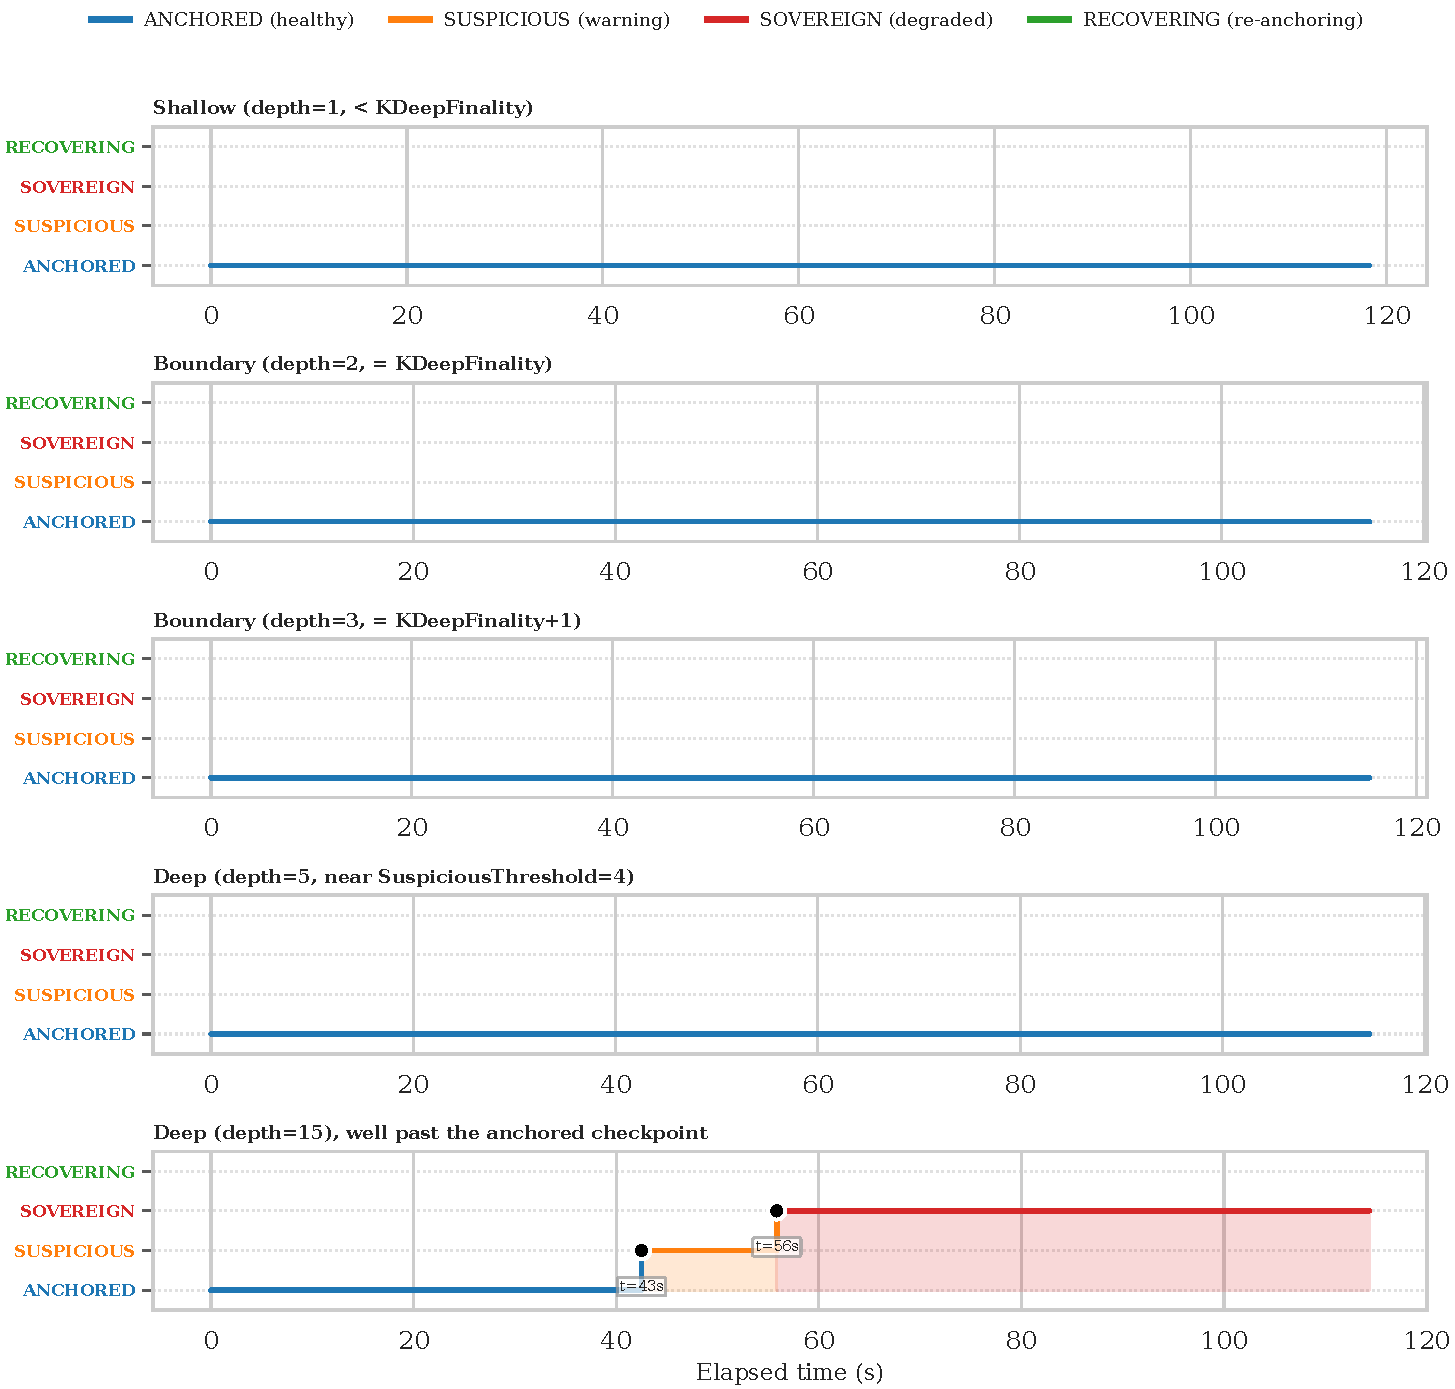
\includegraphics[trim=0 0 0 25pt, clip, width=\linewidth]{figures/figure8_reorg_depth_reaction_live.pdf}
\caption{FSM reaction to Bitcoin reorgs at five depths, one trial per
depth, seven-validator testbed. All 7 validators agree at every one of 181 polled
rounds per trial (1{,}267 samples total, 0 RPC errors).}
\label{fig:reorg}
\end{figure}

\FloatBarrier

Table~\ref{tab:reorg} summarizes the result. Depths 1--5 all orphan real,
independently-confirmed blocks, yet none of them trip the FSM within the
observation window: all 7 validators stay \textsc{Anchored} throughout. At
depth~15, all 7 validators transition \textsc{Anchored}$\to$\textsc{Suspicious}
at $t{=}43$\,s and $\to$\textsc{Sovereign} at $t{=}56$\,s, in lockstep. This
path rules out a direct critical-condition jump: the FSM's \textsc{Anchored}
branch bypasses \textsc{Suspicious} entirely when the committed certificate's
anchor-reverification flag is set, but the observed path instead passes
through \textsc{Suspicious}, and the suspicious-duration counter reached 23 of
the 24-block escalation bound ($\mathrm{MaxSuspiciousTime}$) in the last
sample before the \textsc{Sovereign} transition. The depth-15 reaction is
attributable to this duration-based escalation, not to anchor re-verification
failing.

\begin{table}[h]
\caption{FSM Reaction to Real Bitcoin Reorgs by Depth}
\label{tab:reorg}
\centering
\scriptsize
\begin{tabular}{@{}p{0.16\linewidth}p{0.24\linewidth}p{0.44\linewidth}@{}}
\toprule
\textbf{Depth} & \textbf{Reorg confirmed?} & \textbf{FSM reaction} \\
\midrule
1 (below $K_{\text{DEEP}}$) & N/A (too shallow) & Stays \textsc{Anchored} \\
2 ($=K_{\text{DEEP}}$)      & Yes & Stays \textsc{Anchored} \\
3 ($=K_{\text{DEEP}}{+}1$)  & Yes & Stays \textsc{Anchored} \\
5                           & Yes & Stays \textsc{Anchored} (within window) \\
15 (past checkpoint)        & Yes & \textsc{Suspicious}~(43s) $\to$ \textsc{Sovereign}~(56s) \\
\bottomrule
\end{tabular}
\end{table}

The crossover between depth~5 (no reaction) and depth~15 (reaction) was
not swept at finer granularity. Whether anchor re-verification ever set the
anchor-reverification flag during this run is not established by the
available logs -- the per-validator sensor value was not captured, only the
committed FSM state and suspicious-duration counter. The data that is
available shows the depth-15 escalation came from the suspicious-duration
bound, not from a direct critical-condition jump.

\FloatBarrier

\section{Network Emulation Parameters}
\label{app:netem}

Table~\ref{tab:netem-profiles} lists every \texttt{tc netem} profile, applied
through Pumba. No correlation or distribution option is set, so delay jitter
is uniform and loss is independent per packet (the \texttt{netem} defaults).
Profiles that name no interface use Pumba's default interface
(\texttt{eth0}), which carries Bitcoin, Celestia, and RPC traffic rather than
the dedicated pairwise validator links. Only the S4 scenario and the relay-latency attack (P4) of
Section~\ref{sec:evaluation} target the validator links explicitly.

\begin{table}[h]
\caption{Network Emulation Profiles (Testbed A)}
\label{tab:netem-profiles}
\centering
\footnotesize
\begin{tabular}{@{}p{0.2\linewidth}p{0.4\linewidth}p{0.12\linewidth}p{0.14\linewidth}@{}}
\toprule
\textbf{Profile} & \textbf{Effect and target} & \textbf{Duration} & \textbf{Used by} \\
\midrule
\texttt{chaos-delay} & 100\,ms delay, 20\,ms jitter, all seven validators & 5\,min & baseline \\
\texttt{chaos-loss} & 5\% loss, validators 1 and 2 & 2\,min & composite \\
\texttt{chaos-eclipse} & 100\% loss, validator 1 & 3\,min & S5 \\
\texttt{chaos-btc-delay} & 500\,ms delay, 100\,ms jitter, one \texttt{bitcoind} & 2\,min & composite \\
\texttt{chaos-wan-latency} & Per-validator delay and jitter, Table~\ref{tab:netem-wan} & 10\,min & WAN baseline \\
\texttt{chaos-wan-loss} & Per-validator loss, Table~\ref{tab:netem-wan} & 10\,min & WAN variant \\
S4 eclipse & 300\,ms delay, 50\,ms jitter on the six validator links of validator 1 & 2\,min & S4 \\
P4 relay latency & 350\,ms delay, 50\,ms jitter on all P2P interfaces of one validator & 244\,s & P4 \\
\bottomrule
\end{tabular}
\end{table}

\begin{table}[h]
\caption{WAN Baseline Profiles Per Validator (one profile of seven emulated regions)}
\label{tab:netem-wan}
\centering
\footnotesize
\begin{tabular}{@{}lrrrrrrr@{}}
\toprule
\textbf{Validator} & 1 & 2 & 3 & 4 & 5 & 6 & 7 \\
\midrule
Delay (ms)  & 15 & 70 & 140 & 45 & 100 & 30 & 180 \\
Jitter (ms) & 3 & 15 & 25 & 10 & 20 & 6 & 30 \\
Loss (\%, loss variant) & 1 & 3 & 6 & 2 & 4 & 1 & 5 \\
\bottomrule
\end{tabular}
\end{table}

Each validator receives one delay value on its egress, so the profile is a
per-validator offset rather than a pairwise round-trip-time matrix. A
pairwise matrix between regions is not measured on Testbed~A.
\iftestbedB It is measured on Testbed~B.\fi


\end{document}